%%%%%%%%%%%%%%%%%%%%%%%%%%%%%% -*- Mode: Latex -*- %%%%%%%%%%%%%%%%%%%%%%%%%%%%
%% uhtest.tex -- 
%% Author          : Robert Brewer
%% Created On      : Wed Sep 30 16:08:49 1998
%% Last Modified By: Robert Brewer
%% Last Modified On: Mon Oct  5 16:17:16 1998
%% RCS: $Id: uhtest.tex,v 1.2 1998/10/06 02:04:56 rbrewer Exp rbrewer $
%%%%%%%%%%%%%%%%%%%%%%%%%%%%%%%%%%%%%%%%%%%%%%%%%%%%%%%%%%%%%%%%%%%%%%%%%%%%%%%
%%   Copyright (C) 1998 Robert Brewer
%%%%%%%%%%%%%%%%%%%%%%%%%%%%%%%%%%%%%%%%%%%%%%%%%%%%%%%%%%%%%%%%%%%%%%%%%%%%%%%

%!!!!!!!!!!!!!!!!!!!!!!!!!!!!!!!!!!!!!!!!!!!!!!!!!!!!!!!!!!!!!!!!!!!!!!!!!!!!!!
%!NOTE: This example file has been prepared according to the University of
%!      Hawaii Style & Policy Manual for Theses and Dissertations dated
%!      "Revised February 1998". If you have one with a later date, you may
%!      need to make revisions to this document as well. In any event, making
%!      sure your thesis complies with Graduate Division guidelines is
%!      ultimately your responsibility. Caveat LaTeXtor. :)
%!!!!!!!!!!!!!!!!!!!!!!!!!!!!!!!!!!!!!!!!!!!!!!!!!!!!!!!!!!!!!!!!!!!!!!!!!!!!!!

%% The options are (you can only choose one from each group):
%%
%% 10pt, 11pt, 12pt: chooses the point size for the document. "11pt" is the
%%                   default.
%%
%% oneside, twoside: whether you want your document onesided or twosided. Note
%%                   that twosided is not guaranteed to work, and style
%%                   guidelines prohibit double sided printouts on final
%%                   copy. "oneside" is the default.
%%
%% draft, final: when printing drafts you can save a lot of paper by using the
%%               "draft" option. It switches to single spacing, displays overful
%%               hboxes with a black box, prints a version number on title page 
%%               and omits signature page. Of course for the final copy make
%%               sure to use the "final" option! "final" is the default.
%%
%% cm, times, palatino, newcent, bookman: switches between different font
%%                                        sets. "cm" is the Computer Modern
%%                                        font (TeX's default), the rest are
%%                                        PostScript fonts. "times" is the
%%                                        default.
%%
%% thesis, dissertation: switches between the style for a master's thesis and a 
%%                       Ph.D. dissertation. The differences are fairly minor
%%                       and limited to the front matter. "thesis" is the
%%                       default.
%%
%% actual, proposal: switches between actual document and proposal mode. In
%%                   proposal mode: the title page is simplified, the
%%                   version number is always printed, and the signature page
%%                   is omitted.
%%
%%% Load the uhthesis2e document class
\documentclass[11pt,final,thesis,actual]{uhthesis2e}

%%% Load some useful packages:
%% New LaTeX2e graphics support
\usepackage{graphicx}
%% Support sub-figures.
\usepackage{subfigure}
%% Make subsubsections numbered and included in ToC
\setcounter{secnumdepth}{3}
\setcounter{tocdepth}{3}
%% Package to linebreak URLs in a sane manner.
\usepackage{url}
%% Make URLs clickable
\usepackage[colorlinks, bookmarks=true]{hyperref}
\usepackage[all]{hypcap}
%% Make table cross pages.
\usepackage{longtable}
%\usepackage{tabularx}
\usepackage{array}
%%graphics properties
\graphicspath{{figures/}} 
\DeclareGraphicsExtensions{.eps} 

\def\sectionautorefname{Section}
\def\subsectionautorefname{Section}



%%% End of preamble
\begin{document}

%%% Declarations for Front Matter. Capitalize all of these values
%%% "normally". This allows the document class to format them properly.
%% Full title of thesis or dissertation, capitalized like a title should be.
\title{Learning Empirical Software Engineering Using The Software Intensive Care Unit}
%% Your name, capitalized normally. Do not include any titles like Dr.
\author{Shaoxuan Zhang}
%% Month in which you intend to receive your degree (i.e. graduation).
%% Presumably this will be one of: May, August, or December.
\degreemonth{December}
%% Year of expected graduation.
\degreeyear{2009}
%% Type of degree to be conferred.
\degree{Master of Science}
%% This is the chairperson of your committee. Do not use titles like Dr.
\chair{Philip M. Johnson}
%% The other members of your committee, seperated by "\\". Again, no titles,
%% and it is customary to list the outside committee member (if you have one)
%% last.
\othermembers{Henri Casanova\\
Scott Robertson}
%% This is the total size of your committee, including the chairperson. The
%% signature page routine will only handle up to 6 members; if you have more
%% than that you will need to modify the document class.
\numberofmembers{3}
%% The field in which you are obtaining your degree, capitalized normally.
\field{Information and Computer Sciences}
%% The version number of your document. Consistent use of this will enable you
%% to tell old drafts from new ones. Final actual documents omit this
%% automatically so you can use it without fear of submission problems at the
%% end. If you do not define this parameter, it defaults to "1.0.0".
\versionnum{0.5.0}

%%% Create the title page from all the information above. Note that the
%%% titlepage is outside the front matter.
\maketitle

\begin{frontmatter}

%%% Create the signature page (when indicated by the options)
\signaturepage

%%% Create the copyright page
\copyrightpage

%%% Bring in the dedication page from external file

\begin{dedication}
\null\vfil
{\large
\begin{center}
To my mom, dad, wife, and my new born baby girl Ruby.
\end{center}}
\vfil\null
\end{dedication}


%%% Bring in the acknowledgments section from external file

\begin{acknowledgments}
I want to ``thank'' my committee, without whose ridiculous demands, I
would have graduated so, so, very much faster.
\end{acknowledgments}


%%% Bring in the abstract section from external file

\begin{abstract}
In software engineering, the importance of measurement is well understood, and many efficient software development metrics have been developed to help measurement. However, as the number of metrics increase, the effort required to collect data, analyze them and interpret analysis results quickly becomes overwhelming. This problem is even more critical in educational approaches regarding empirical software engineering.

The Software Intensive Care Unit is a new approach to facilitate software measurement and control with multiple software development metrics. It uses the Hackystat system to achieve automated data collection and analysis, then uses the collected analysis data to create an intensive monitoring interface for multiple ``vital signs''. A vital sign is a wrapper of a software metric with proper presentation. It consists of a historical trend and a newest state value, both of which is colored according to its ``health'' state. I hypothesize that the Software ICU is helpful to study empirical software engineering.

My research deployed and evaluated Software ICU in a senior-level software engineering course. Students' usage was logged in the system, and a survey was conducted. The results provide supporting evidence that Software ICU does help students in course project development and project team organization. In addition, the results of the study also discover some limitations of the system, including inappropriate vital sign presentation and measurement dysfunction.

\end{abstract}


%%% Generate table of contents
\tableofcontents

%%% Generate list of tables
%\listoftables

%%% Generate list of figures
\listoffigures

\end{frontmatter}

%%% Bring in the body of the thesis from external file

\chapter{Introduction}

%In large companies, it is possible to have dozens or even hundreds of software projects underway at any given point in time. This kind of scale produces new challenges, as well as new opportunities for these companies. Both challenges and opportunities result from the need of the company to successfully understand and exploit their ownership of a portfolio of software projects. 

%Single project management is easy to achieve from various way. Many software metrics, such as coverage, complexity and file size, provide significant information about a software project. But it is reported that, almost all metrics have deficiency when judge a state of a project with only one or two of them. Therefore, people usually trend to look into more metrics to understand a project. However, while the number of projects increases as well as the number of metrics increases, the data to read inflates rapidly and become overwhelming.

%In order to address this issue and achieve efficient governance over large number of projects, we introduce an analysis tool called Software Intensive Care Unit. It is from the idea of intensive care unit in hospitals where patients are placed with sensors from sophisticated machines and they are consistently monitoring the patients' various vital sign such as pulse, breathe, etc. Similarly, Software Intensive Care Unit(SICU) provides various software metrics, each of which reveals one aspect of the project. These metrics are the vital signs of a software project. With all these vital signs together, users can have a fast but complete view of the projects, leading to easier understanding of projects and make better decisions and practice. Though one might argue that software projects' performance cannot be simply judged by a set of metrics, the case is the same in medicine. A doctor will not simply diagnose a patient by those vital signs, but it is undoubtedly that the medical intensive care unit helps the diagnosis a lot, so it is the software intensive care unit.

%However, to build up the SICU is a great challenge. Both what data to show and how to show them are essential to successfully set up a SICU that offer enough insight into the most interesting aspect of the projects without too much data overwhelming. Moreover, interesting things are various from different situation. Some setting may be common over projects and organization, but we don't believe there is a golden rule for all projects. So system should give users the capability to customize as their need.


\section{The Problem}
Software metrics are the essential tool for performance measuring and quality control. But they are not comprehensive enough to make judgement with only one or two. So, we need to utilize multiple metrics in order to acquire insight of the health state of the software project. The more software metrics, the more comprehensive insight, but also the more effort is required to collect measure data and interpret values. My research tries to overcome this challenge by developing a system to help observe the health status of the software project from multiple software metrics in an effective way.

\section{Software Intensive Care Unit Approach}
What is SICU

\section{Thesis Claim}
We claim it is the most powerful tool ever in the world! =P

\section{Evaluation}
We evaluate in a classroom.

\section{Thesis Structure}
Here is a paragraph that saying the same thing as TOC.

\chapter{Related Work}
This chapter presents some works relate my research.

First part discusses previous research on empirical software engineering concepts. Most previous researches on measurement-based software engineering focus on methodology. Effective approaches are developed and deployed in actual practice. However, the lack of automation adds significant overhead to developers, thus lead to the impression that they are hard. Research of Hackystat and Software ICU is towards the 3rd generation of approaches to PSP metrics that automate data collection and analyze\cite{csdl2-02-07}.

Second part discusses three recent research that focus on automated data collection. Two of them mainly focus on introductory level programming course and not very suitable to senior software development or professional settings. The third one is very similar to Hackystat and has related industry studies.

%Third part discusses some commercial ``dashboards'' for software project data. Software ICU is one example of a project dashboard. However, it differs from commercial approaches with its intensive metrics, high extensibility and open source development and distribution. 

Last part discusses two previous related case studies of Hackystat system to provide some insight into the development history of Hackystat.

\section {TSP/PSP}
The Personal Software Process(PSP)\cite{book:psp} and the Team Software Process(TSP)\cite{book:tsp} are among the most extensively studied approaches for measurement-based software engineering. They were developed by Watts Humphrey to teach students (in university and industry alike) the use of large scale methods based on the Capability Maturity Model (CMM). They scale down industrial software practices to fit the needs of small scale program development. Software processes and software engineering disciplines are gradually introduced through small program projects (e.g. course assignment projects). The PSP maturity progression is shown in \autoref{fig:PSP-Evo}. Students gather both process and product measures of their projects. By comparing the measurement result to their original planning, they comprehend their programming habits, both pros and cons, and refine their process to higher level of maturity.

\begin{figure}[htbp] %  figure placement: here, top, bottom, or page
   \centering
   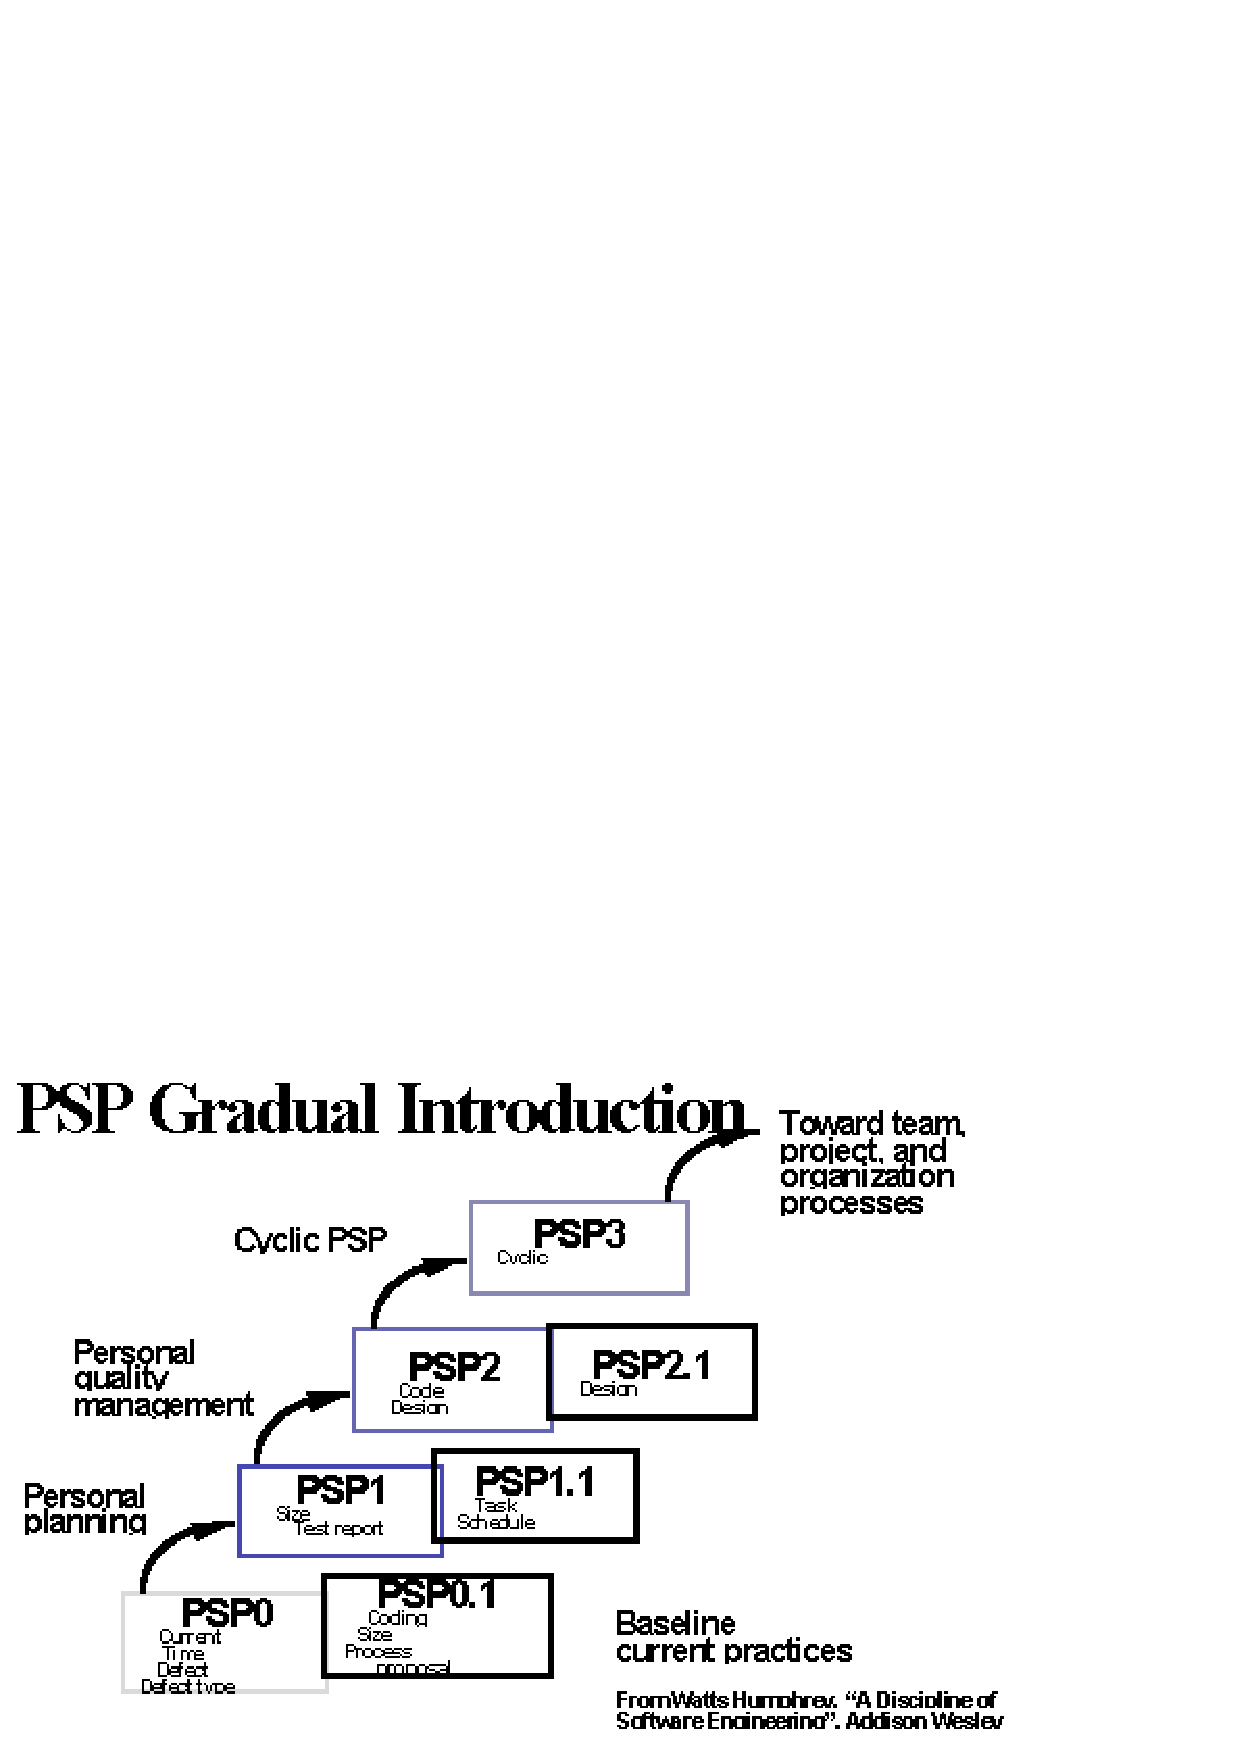
\includegraphics[height=20em]{PSP-Evo} 
   \caption{Progression of PSP}
   \label{fig:PSP-Evo}
\end{figure}

%PSP/TSP is effective in both academic education as well as industrial application. (more about related research)

Their major drawbacks are lack of automation. Developers have to manually record their process and product data (mostly the development time and number of defects). The high overhead of data collection raises a barrier to its introduction and adoption. Additionally, it is not easy to ``digest'' the data. Developers have to manually analyze their logged data in order to understand the their performance, then be able to improve it.

On the contrary, Software ICU provides a higher level of automation in tracking and analyzing software process and product data.


\section {Research Based on Automated Data Collection}
Project ClockIt and Retina are two recent research based on automated data collection to support entry-level programming courses, while PROM is the most similar research to Hackystat.

\subsection {Project ClockIt and Retina}
Project ClockIt provides a data logger as BlueJ\footnote{``BlueJ is an integrated Java environment specifically designed for introductory teaching.'' --Quoted from \url{http://www.bluej.org/about/what.html}}
 extension. It logs developer's open/close of project and package, file change and delete and compilation results. Data is logged to local file and later sent to a database via Internet. A data visualizer integrated into BlueJ is available to view data about the current project. \autoref{fig:clockit} shows an example of this visualizer. Data stored in database is used for statistic analysis such as class averages. A web interface is also available to instructors to view the individual data of their students and class average analysis data.

\begin{figure}[htbp] %  figure placement: here, top, bottom, or page
   \centering
   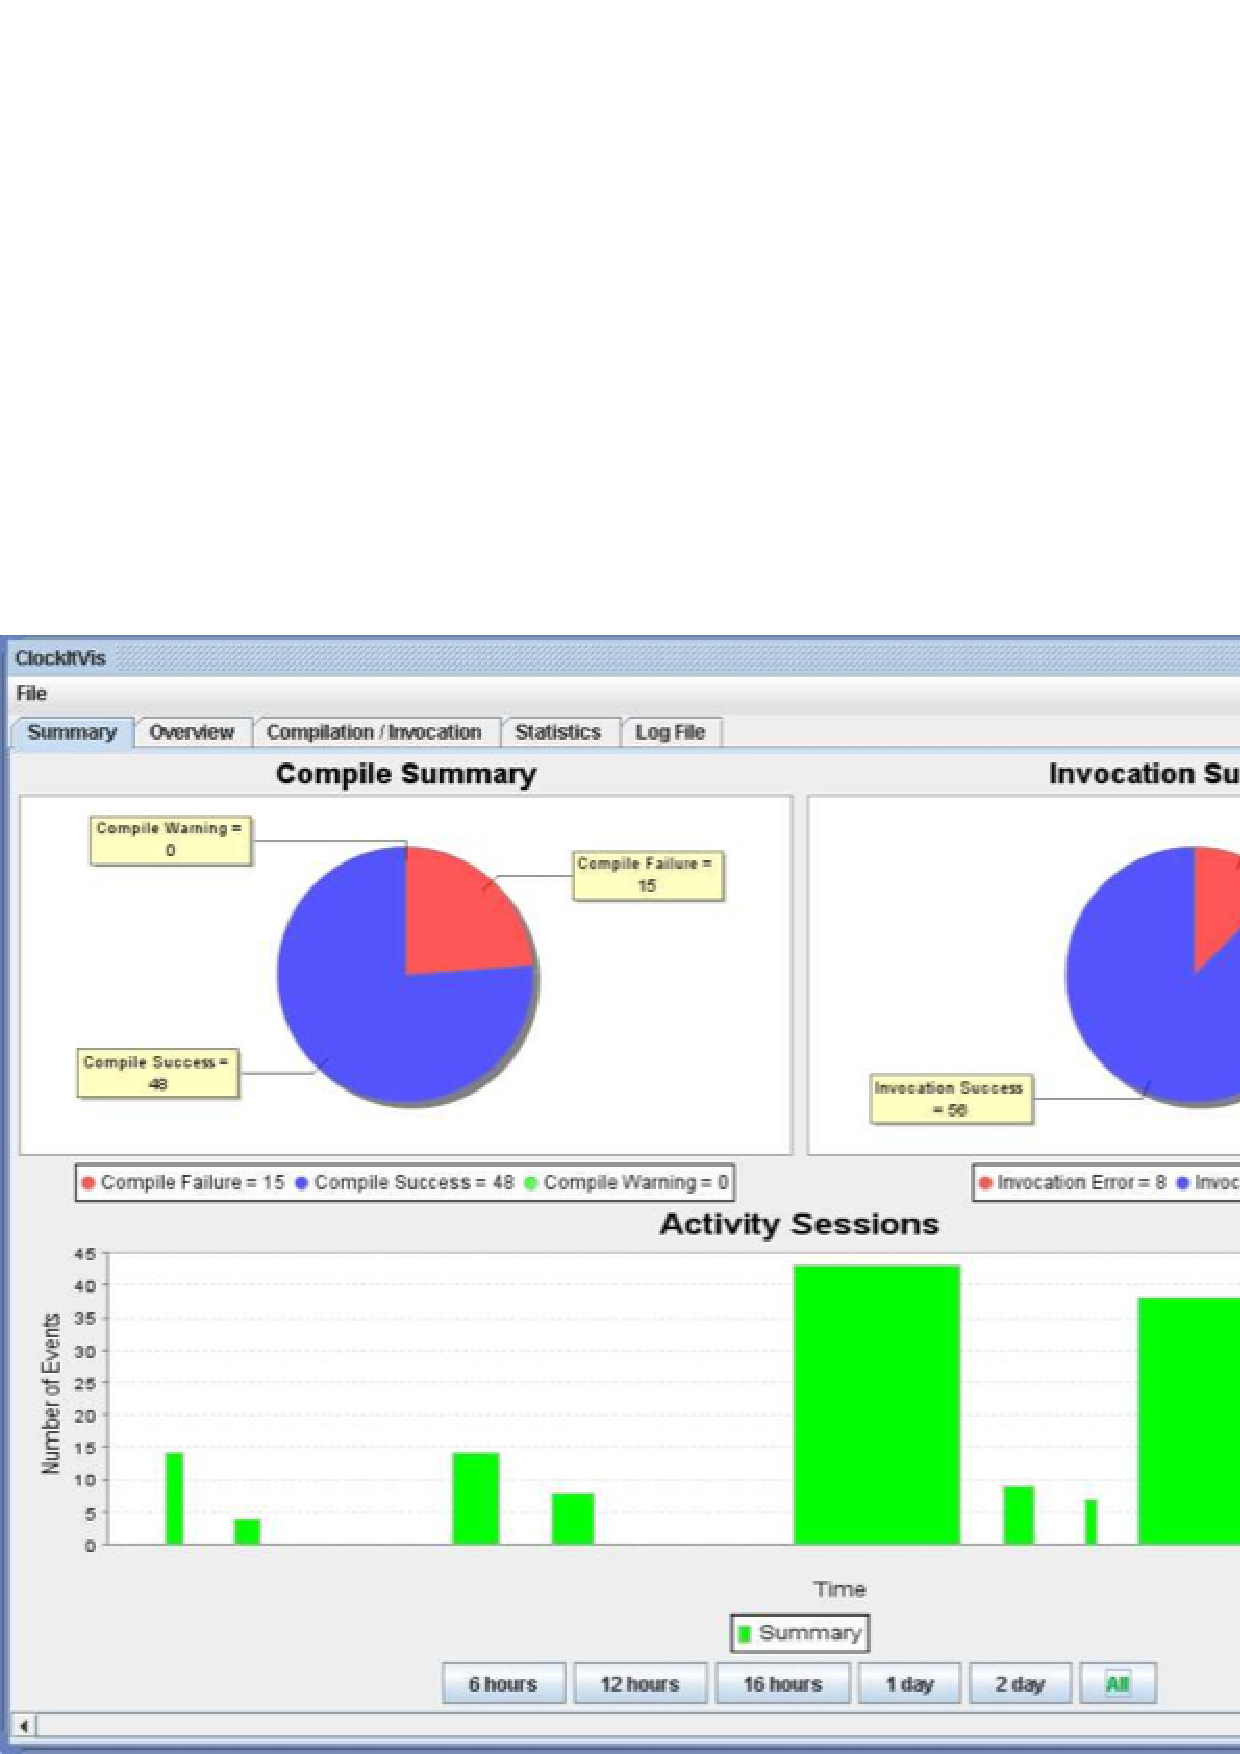
\includegraphics[height=20em]{clockit} 
   \caption{ClockIt BlueJ Data Visualizer summary}
   \label{fig:clockit}
\end{figure}

Closely related to ClockIt, Retina also provides automated data collection. Though Retina provide more tool support (BlueJ, Eclipse and command-line compiler), it focuses on a even smaller area of programming events: compilation. It gather data from students' compilation events, mostly compilation errors. In additional to its data viewer (see \autoref{fig:retina}), it also provides a recommendation tool for students. The tool use instant messaging (IM) to give students recommendation of approximated time needed for the upcoming assignment, and the compilation errors one is likely to make. These are based on both the student's previous data and the data from courses of previous semesters. 

\begin{figure}[htbp]
     \centering
     \subfigure[Retina Instructor Viewer]{
          \label{fig:retina-teacher}
          \includegraphics[width=.48\textwidth]{retina-teacher}}
     \subfigure[Retina Student Viewer]{
          \label{fig:retina-teacher}
          \includegraphics[width=.48\textwidth]{retina-student}}
          
     \caption{Data viewers of Retina.}
     \label{fig:retina}
\end{figure}

The difference between these two research and Software ICU is that they focus only on introductory level courses, where compilation is the interesting development event. In other hand, their relatively easy configuration overcomes one of the major short-coming of Hackystat and Software ICU. While neither of them provide good extensibility, they are unlikely to be useful in advanced programming situations like advanced programming course or professional setting.

\subsection {PROM}
PRO Metric (PROM) \cite{prom03} is a system that similar to Hackystat. PROM is a software system for collecting process and product metrics in a software company. It is initiated and driven by the demand of the company, and thus the research is focus on industry setting. It is designed to work fully automatically without any interaction with the user in order to get reliable and accurate data about company internal workflows and development processes. It is organized in a sequence of interconnected components, communicating using SOAP protocol. Similar to sensors in Hackystat, it has plugins for many different applications, including IDEs, word processing tools, email clients, and issue tracking systems. Data then is transit to plugin server to extract metric, then the results are sent to PROM server to store into database. \autoref{fig:promarchitecture} shows the overview of PROM's architecture.

\begin{figure}[htbp]
     \centering
     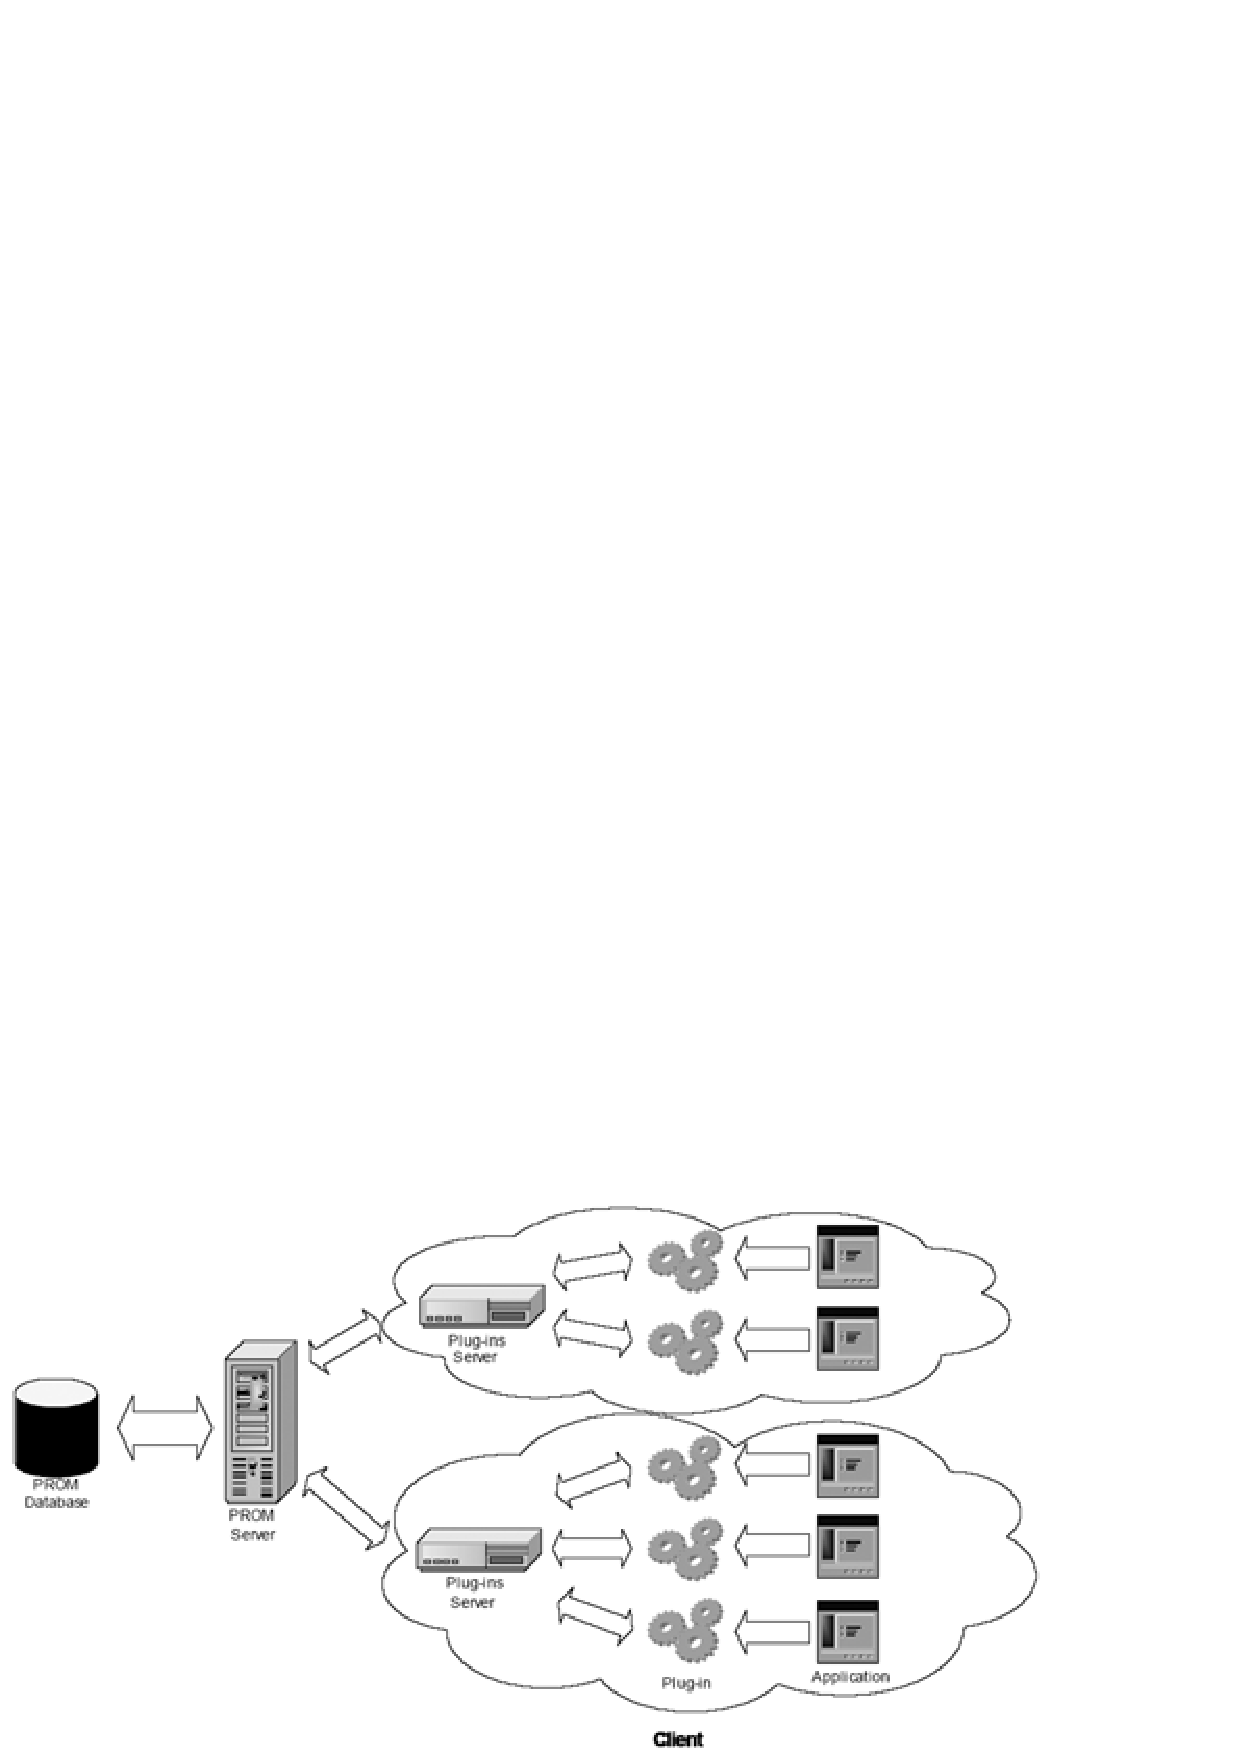
\includegraphics[width=.48\textwidth]{promarchitecture}
     \caption{Architecture of the PROM system}
     \label{fig:promarchitecture}
\end{figure}

PROM categorize users into 3 roles, developer, team leader, and manager of the team. Each of these role is provided different views of data. Developers have access to their individual, detailed data, the leader to the aggregated data of the whole team, and the manager to project level aggregated data.

Compared to Hackystat, PROM's data is stored as analyzed metrics result while Hackystat stores the raw sensor data. Different data viewers are provided to different groups of users while Hackystat provides same viewers to all users.

A case study of PROM in industrial environment\cite{prom09} discusses the lessons learn from two year experience of using the PROM system in the IT department of a large company in Italy. Evidence indicates that adopting the PROM system requires a long set-up phrase and need the company and develop team's patience and commitment to succeed, but it eventually delivers value to the company. 

One of the lessons suggest that data presentation is as important as data accuracy and simplicity, brevity and clarity is preferable. Another lesson suggest that fast aggregated view of data is desired, and users of different roles favor different aggregations, e.g. developers like reports of their daily activities, while team leader and manager like summary views of data on team and project level. Software ICU's simple and fast data presentation and high configurability and extensibility is suitable to address these requirements.

%\section {Software Project Dashboards}
%In software industry, there exists many commercial software project manage dashboards, such as LightHouse, ProjectManager.com dashboard, PivotLink Dashboards, Autotask Project Management and so forth. However, many of them are complete solution of software development business management, including not only software project states management, but also related resource allocation and budget control, etc. As being commercial products, they are not open source. Most importantly, there is few research published about these commercial project dashboards. ``Features'' are advertised as other commercial products, while short-comings are ignored. Thus negative results of their use are unknown. This research of Software ICU contains not only its benefits, but also its negative impact.


\section {Previous Case Studies of Hackystat}
The classroom study presented in this thesis is the third case study of Hackystat system in a classroom setting. 

The first case study performed in 2003 used an early version of Hackystat\cite{csdl2-03-13}. During that time, Hackystat was only collecting 4 types of metrics (Active Time, Size, Unit Tests and Coverage). The system was oriented around a set of ``Course'' analyses that were tailored to an educational setting. Those analyses summarize the individual team project metric data in tabular form, and also presented comparisons of all of the course projects\autoref{fig:hackystat2003}. The evaluation show that the installation of Ant sensors is the most significant barrier to the system. It was too difficult to install without direct help from the development team. But the overhead of use is relatively low and analyses were usable and useful. Data privacy was uncomfortable for some students.

\begin{figure}[htbp]
   \centering
   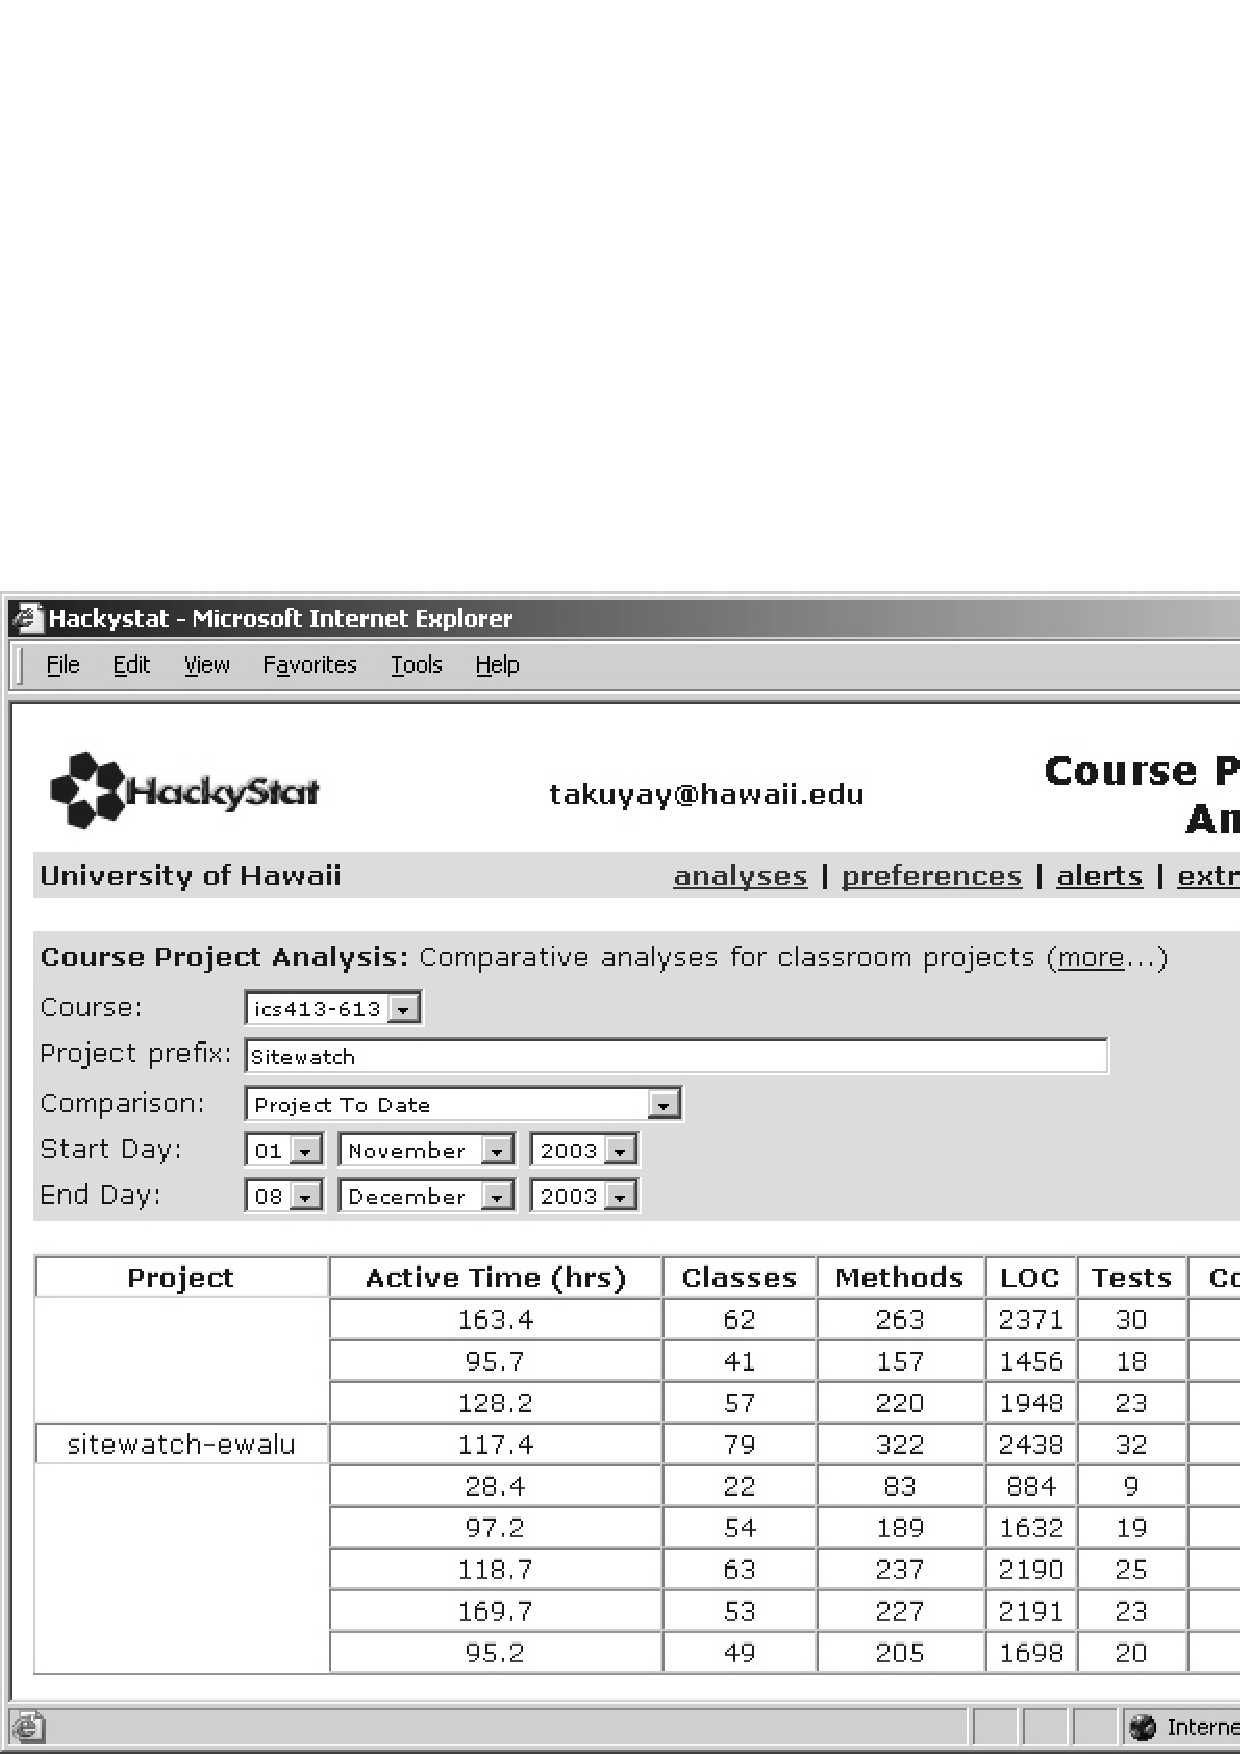
\includegraphics[height=20em]{hackystat2003} 
   \caption{Screenshot of course project to date analysis of Hackystat in 2003}
   \label{fig:hackystat2003}
\end{figure}

The second case study in 2006 is a partial replication of the first case study\cite{csdl2-07-02}. Hackystat had undergone significant change from 2003 to 2006. The sensor installation, which is the major barrier to the system in 2003, was automated by the hackyInstaller GUI, which greatly lower the overhead of configuration for developers. The evaluation also shows significant drop in sensor installation difficulty. However, new sophisticated Telemetry analysis \autoref{fig:hackystat2006} and its complex user interface raise the difficulty of using it and interpreting data, lead to slight drop in usability and professional feasibility.

\begin{figure}[htbp]
   \centering
   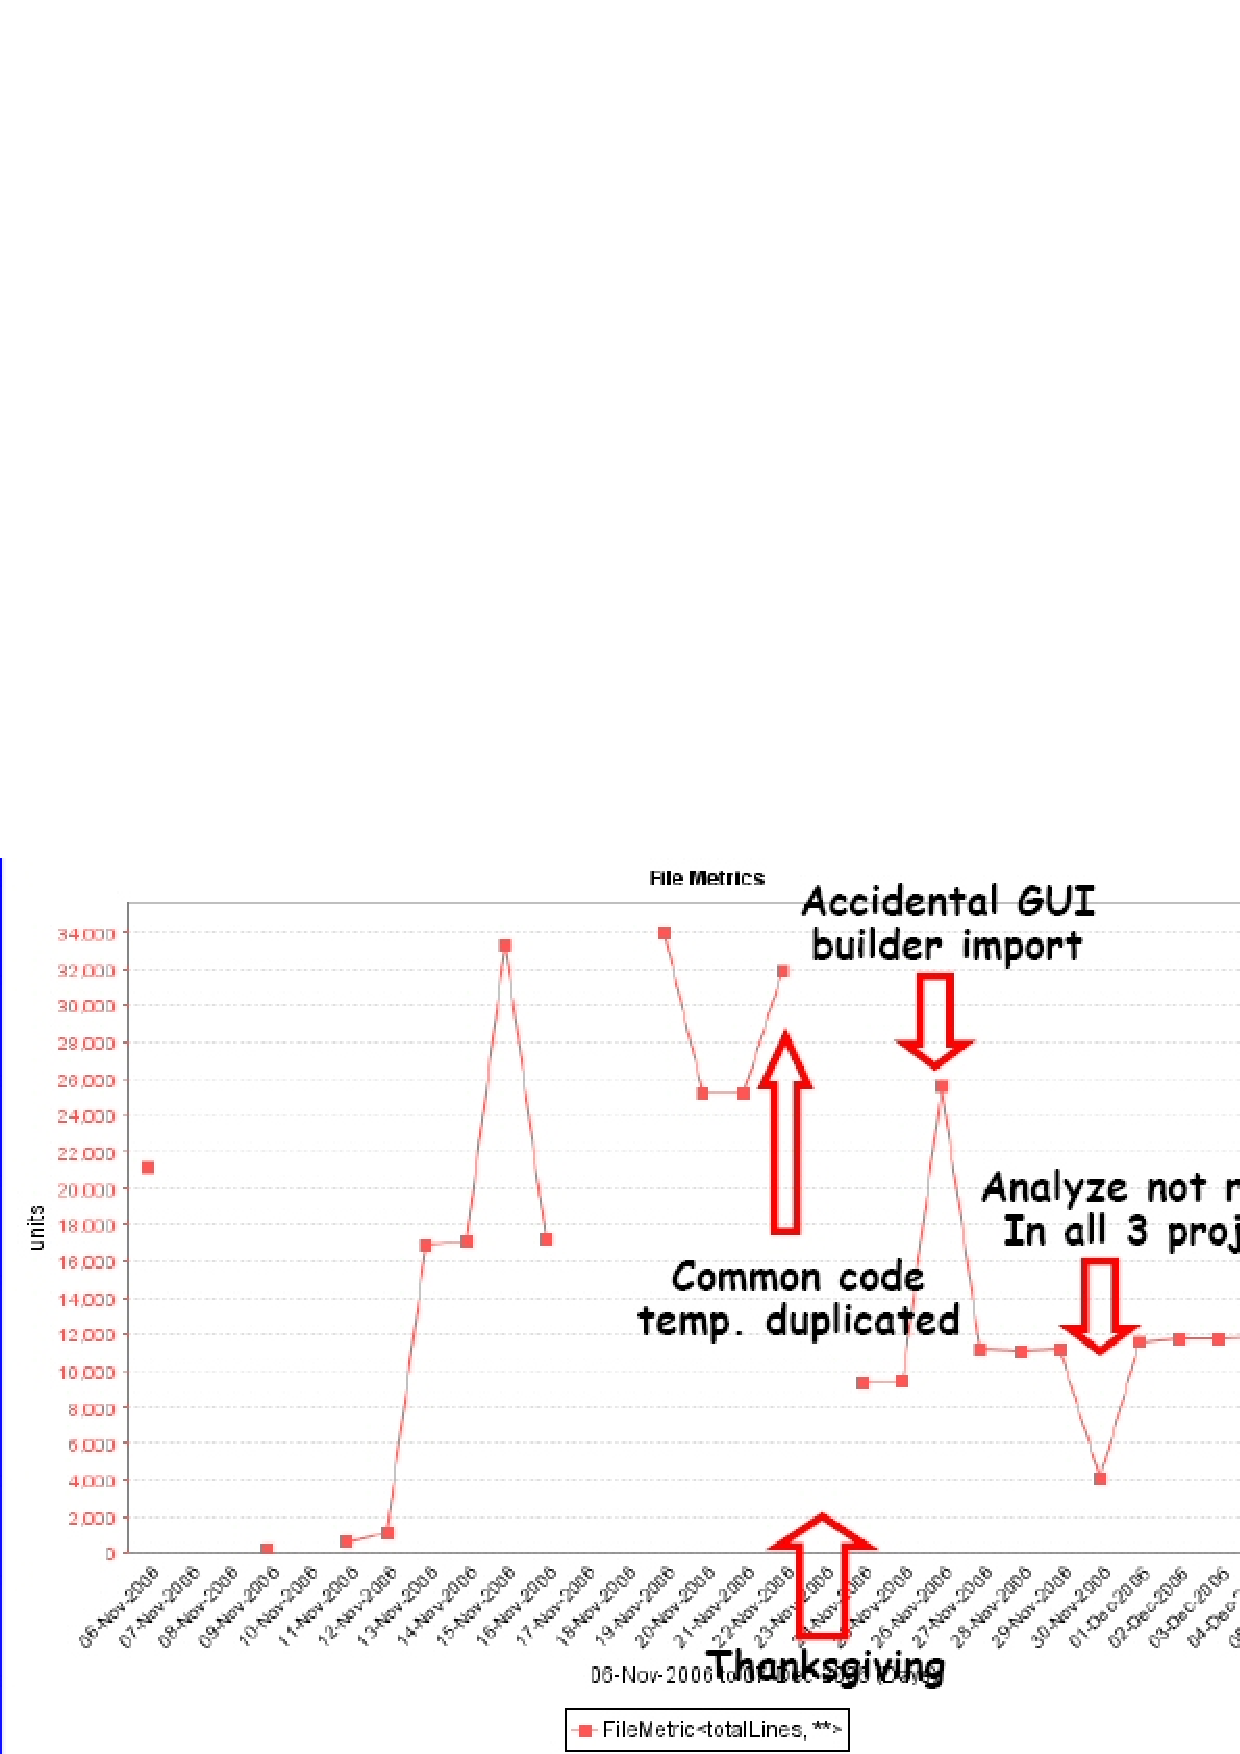
\includegraphics[height=20em]{hackystat2006} 
   \caption{Screenshot of file-metric telemetry analysis of Hackystat in 2006}
   \label{fig:hackystat2006}
\end{figure}

In 2007, Hackystat was re-implemented using a new architecture. Adopting service-oriented architecture enable  multiple user interface separate from the services components. The Software ICU is built upon a new web-based UI called Project Browser, and the classroom study is also based on this user interface.


\chapter{Hackystat}
In this research, I utilize Hackystat to implement the Software ICU. This chapter briefly introduce the Hackystat system, which was invented by Professor Philip M. Johnson, in the Collaborative Software Development Laboratory, Department of Information and Computer Sciences, University of Hawaii at Manoa. 
 
\section{Hackystat Framework}
Hackystat is an open source framework for collection, analysis, visualization, interpretation, annotation, and dissemination of software development process and product data. Hackystat consist of many software services that communicate using REST architectural principles\cite{wiki:restful}. These software services can be categorize into 4 groups, sensors, data repository, analysis services and viewers. \autoref{fig:hackystat-architecture} shows the architecture of Hackystat system. 

\begin{figure}[htbp]
   \centering
   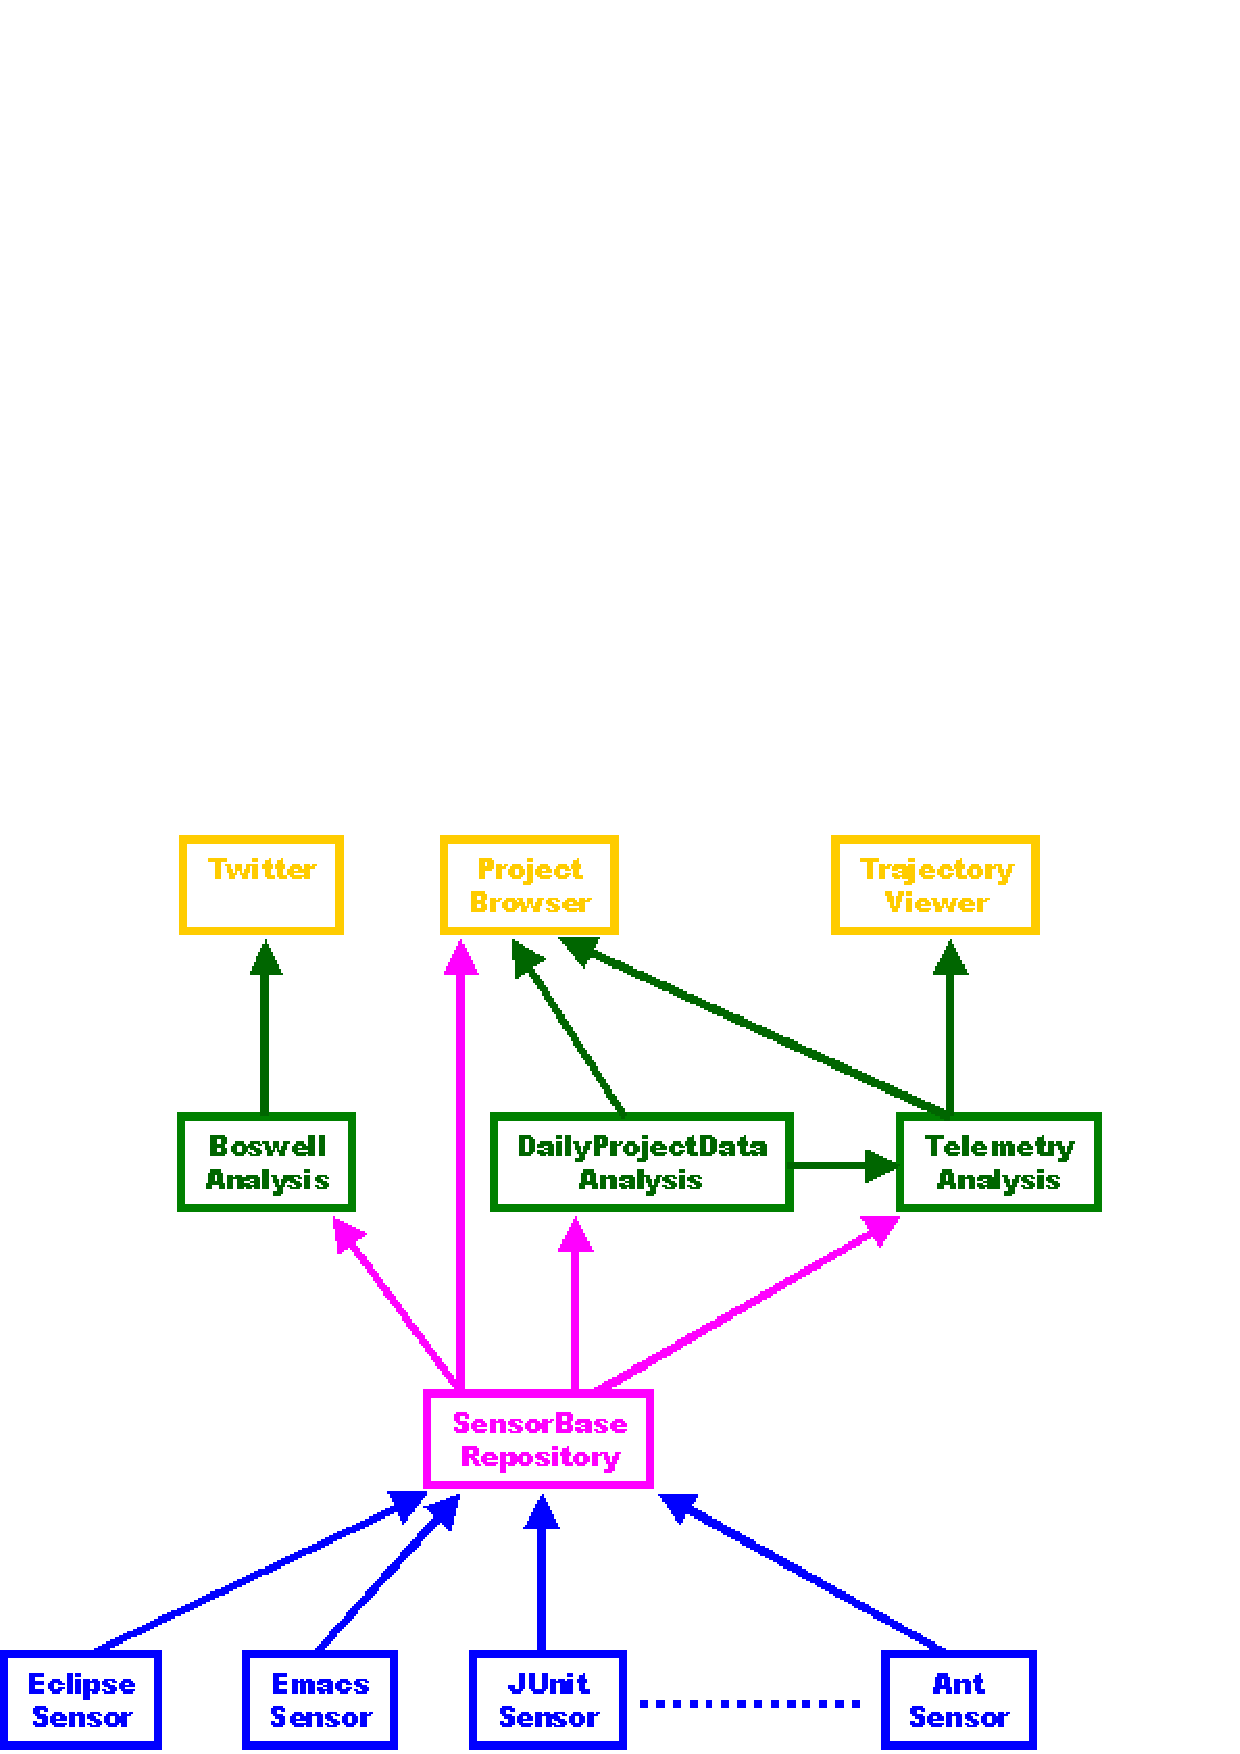
\includegraphics[height=20em]{hackystat-architecture} 
   \caption{Screenshot of file-metric telemetry analysis of Hackystat in 2006}
   \label{fig:hackystat-architecture}
\end{figure}

\subsection{Sensors}
Sensors are small software plugins that collect data from the use of tools and applications. Currently, sensors are available in many development software including Eclipse, Emacs, Ant, etc. Sensor data is represented in XML, and consist of seven basic elements: data owner, resource, timestamp, runtime, tool, Sensor Data Type and properties. The first six are required and the last one is optional. 

Sensor Data Type(SDT) is specified in every piece of sensor data when collected, so that the same type of data can be collected from different tools and higher level services can easily determine which data is relevant to them. Sensor data is designed to record only an piece of atomic data such as size of a single file, and runtime is use to group data that belongs to the same event, such as the file metric of a project. Properties are additional information for different types of sensor data, such as coverage value for coverage SDT and lines of code for file metric. 

Sensors are designed to work automatically without any attention of user besides initial configuration. In order to reduce internet communication and support offline work, data is temporarily stored, then sent to data repository every several minutes or when internet connection is available.

\subsection{SensorBase}
Sensor data is sent to the data repository, called SensorBase. SensorBase store the data as it sent from sensors, and provide RESTful interface for easy use. Sensor data can be queried with the six required elements mentioned above via HTTP calls, and data is sent back as XML. SensorBase is implemented with a database manager abstract class, thus it is easy to add support to different database implementations. Current version of Hackystat provides database support for Derby, Oracle and PostgreSQL.

\section{Analysis Services}
Analysis services of Hackystat provide abstractions of the raw data from SensorBase. DailyProjectData and Telemetry are the two most fundamental analyzes of Hackystat.

\subsection{Daily Project Data Analysis}
As its name says, DailyProjectData(DPD) service provides abstractions of sensor data associated with a single project within a 24 hour period, which represents a simple software development metric of a single day. Data of a single project includes data from all members of that project. In a DailyProjectData instance, both summary value, e.g. total development time across the project, and detail values, e.g. total development time of a project member, are available. So it is easy for higher level service to use this data.

Each DPD analysis generates software metric from data of a certain Sensor Data Type. Current available DPD analyses are Build, Code Issue, Commit, Complexity, Coupling, Coverage, Dev Time, File Metric, Issue, and Unit Test. These DPD analyses are the basic of the Hackystat system, all other analysis services are based on DPD. While DPD is the lowest level of abstraction, these can also be considered as the available software metrics in Hackystat.

\subsection{Telemetry Analysis}
Based on DPD service, Telemetry service provides abstraction over a longer period of time such as several days, weeks or months. A Telemetry Chart consists of one or more streams of data points. Each data point represents the metric value of in a single granularity (day, week or month). Together they show the trend of the metric(s).

There is a special group of Telemetry charts called Member-Level Telemetry. These charts consist of several stream, each of which belongs to a project member. They are used in Software ICU's drill down feature to compare performance of each member within a project. 

To support the work practices of different organizations, Telemetry service provides a domain specific language that allows to build new Telemetry Chart with Telemetry stream lines. The predefined Telemetry Charts are all written with this language.

Telemetry streams can also accept parameters to refine the object data. This feature is inherited in Software ICU, where user can configure the parameters of each Telemetry analysis of each vital sign (more detail discuss in \autoref{vitalSign} and \autoref{SICUconfiguration}).

\section {Project Browser}
Project Browser is one of the viewers in Hackystat system. It is based on Wicket\footnote{\url{http://wicket.apache.org/}}, a Java-based web application framework. Project Browser is integrated with viewers to all Hackystat services, which are organized as tabs. 

With help of Wicket's modularization, viewers on Project Browser can share many common panel, such as project/date selection panel and Ajax loading process panel, which facilitate the development of new page. This also makes user's experience more consistent across different viewers. Therefore it now serves as a data presentation and high level analysis development center. Several new presentations and high level analysis are developed upon it, Software ICU is one them.

\chapter{Design and Implementation of Software ICU}
In order to achieve good governance of software development projects, we adopt the metaphor from medical ICU and develop a system called Software Intensive Care Unit. It consists of a set of vital signs, each of which is based on one software development metric and indicates the project's ``health'' state from one perspective.

Interface of Software ICU is separated into two part. The left-hand side is the control panel, where user can pick the analysis period, data granularity and select projects to analyze. The right-hand side consists of three panels: the data panel, the loading process panel, and the configuration panel. Each of these panels is discussed in following sections. Data panel is the major panel to show the result of SICU analysis. \autoref{fig:overview} shows an example of Software ICU.

\begin{figure}[htbp]
   \centering
   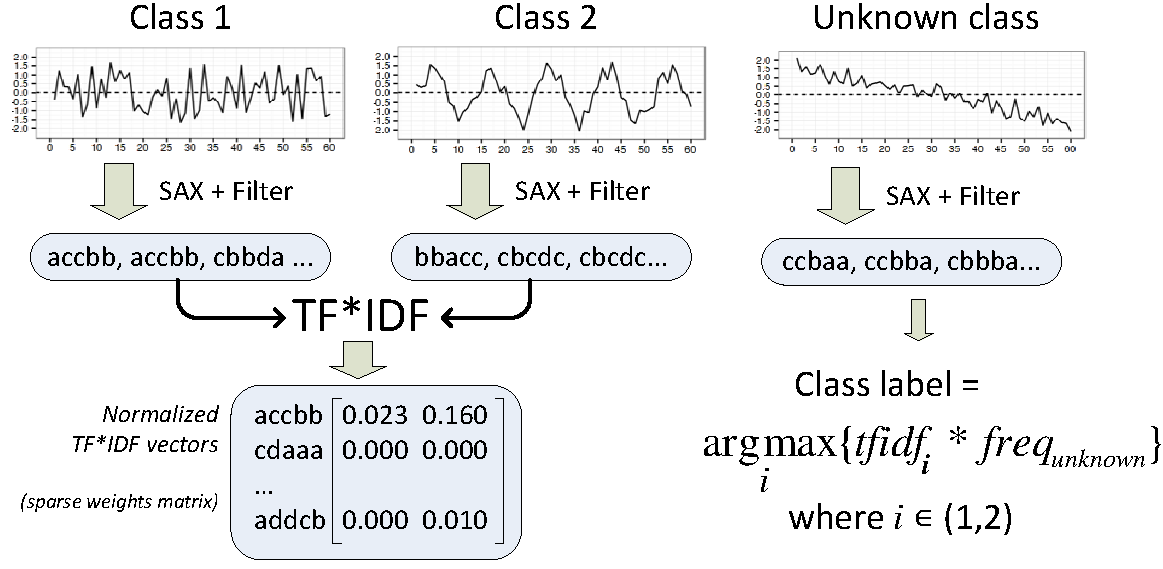
\includegraphics[width=\textwidth]{overview}
   \caption{A screenshot of Software ICU}
   \label{fig:overview}
\end{figure}

\section{Vital Signs}
\label{vitalSign}

Similar to medical ICU, using multiple software development metrics in Software ICU are necessary because there is not a single metric can determine the health state of a software project. Similar to medical vital signs, each software metric show the process or product state from different aspect. And changes in one of them may or may not indicate a change in health state, but changes in more of them indicates higher possibility that health state changed. In this study, we use nine vital signs in Software ICU.

Vital signs of software projects are measured by various software development process or product metrics. Each of these vital sign reveal an aspect of the health state of the software project. In this section I will discuss all these vital signs.
\begin{description}
\item[Coverage] 
Coverage is a good indicator of the tests' quality. It stands for the test coverage of source code in unit testing, which usually measured as the percentage of code units (line, method, class, etc) that is executed during unit test. There are a number of coverage criteria, such as line, method, class, conditional, etc. In Software ICU, user can select which to use. No matter which criteria to use, higher coverage is always better because higher percentage of code covered by unit testing indicates lower risk of existence of bug in untested code segment. However, high coverage does not necessary mean good quality of unit test, and vice versa. One of the reason is that, in some situations, it is difficult to achieve high test coverage because of the difficulty of verifying results, especially when using UI frameworks. Another reason is that the code executed during unit testing can be unverified. For example, when testing an image processor with a given image file, the code of loading the image file is executed, but the test does probably not have assertion about the correctness of loading the file. But as long as developers don't have the intend to trick coverage in order to pretend to be writing enough unit tests (It is possible if coverage is used to judge their performance.), raising coverage is always a good thing.

\item[Cyclomatic complexity] 
Cyclomatic complexity, a measurement of the complexity of a program developed by Thomas J. McCabe, measures the number of linearly independent paths through a program's source code\cite{mccabe:complexity}. The higher cyclomatic complexity, the more distinct control paths in a program module, and the more difficult to achieve high path test coverage. Additionally, code of high complexity is difficult to understand, thus it is hard to maintain. Therefore, program modules are preferred to have lower complexity. But high complexity is not necessary evil. The nature of some programs just require high level of complexity. Also raising in complexity is sometimes unavoidable during development, especially when optimizing code performance. However, developers should try to lower complexity, especially in early stage of development, so that it is easier for future maintenance.

\item[Coupling] 
Coupling, or dependency, is the degree to which each program module relies on each one of the other modules\cite{wiki:coupling}. It is a measurement of the complexity of the whole system's module reference tree. Whenever one module is modified, there will be a chance that the changes may cause bugs in one of modules that relies on it. Therefore, higher coupling implies higher risk of introducing bugs when making changes, thus harder to maintain. High coupling might also be harder to reuse because dependent modules must be included. Therefore, Coupling is suggested to be kept low.

\item[DevTime] 
DevTime, abbreviation of Develop Time, is a measurement of develop time of developers. Hackystat use a special approach to measure this: for each 5 minutes interval, if there is anything development activities happen, the developer is consider developing in that interval. It relax the criteria of measuring develop time so that coding while reading from documentation will get the same DevTime as intensive coding period. Thus it is more accurate than previous ActiveTime in older Hackystat. However, Hackystat sensors for DevTime are only available in several IDEs (currently available to Emacs, Eclipse, and Visual Studio). No sensors are available for other applications that might be used during developing, such as browsers, E-mail clients, office systems, or other editors/readers. So the monitored development activities is limited. Moreover, some developing activities, such as reading and learning, are very difficult to track. Therefore, DevTime should not be simply used to determine a developer's effort. But as habit of an individual will not change a lot, so the DevTime of a developer should be relatively stable over time. Thus large sudden increase in DevTime is a possible sign of bad developing habit like ``start late near deadline''.

\item[Churn] 
Churn is a measurement of the change (add, delete and/or modified) of code that is made into repository. It is usually measured by LOC (lines of code). It is an indicator of developers' contribution to the project. Interpretation of this metric is conditional. In the early stage of development, churn is expected to be higher because new codes are keep being added. During the maintenance of a system, churn is mainly from fixing bugs and adding new features, both of which are fewer for a stable system, thus churn is expected to be lower. In terms of develop behavior, churn of a developer reflects the amount of work of him/her. It tends to be relatively stable over time in the same project because the work rate of an individual does not vary a lot in the same coding condition. Dramatically change in churn of an individual developer while DevTime not changing respectively is a bad phenomena, which might due to bad developing habit like ``copy and paste without understanding''.

\item[Commit] 
Commit measure the number of commitments made into repository. ``Commit early, commit often'' is one of the well-accepted guideline of continuous integration. For the same amount of churn, more commits implies better following of this discipline.

\item[Size] 
The size of the project is measured by the source lines of code (SLOC), which counts the number of lines in the text of the program's source code. It can be a sign of the effort put into the project, However, SLOC alone does not make as much sense about the state of the project as Churn. We include this vital sign only to give user an idea of the size of the project, just like the height in your medical record.

\item[Test] 
Test is a count of unit test tasks invoked in a period of time. Unit testing is a software verification and validation method in which a developer tests an individual units of source code. It is used to ensure that code meets its design and behaves as intended. A requirement of good development behavior is to test while coding, or event better, use ``Test Driven Development'' (TDD). No matter what development pattern to follow, unit testing is a dispensable component and regular execution of unit tests is always a good sign of ``health'' development habit.

\item[Build] 
Build is a count of ant build task invoked in a period of time. A build task accomplish all necessary step to ensure the correctness of the code before commit. It consists of compilation, code inspection, unit testing, documentation generation, etc. It is an usual activity in software development nowadays. Though how often to build largely depends on personal preference and habit, it is advised to build often to ensure the correctness of the system.

\end{description}

These nine vital signs are the default set in Software ICU, but not the only setting. Users can determine to use which vital signs in their setting, as well as creating new vital sign analysis with Telemetry charts. More detail about these configuration and customization are discuss in \autoref{SICUconfiguration} and \autoref{SystemCustomization}.

\section{Vital Sign Presentation}
As reported in case study of PROM, data presentation is as important as data accuracy\cite{prom09}. One of our primary goal of Software ICU is to provide a proper presentation to help interpret large amount of software metrics data. In order to achieve this goal, Software ICU use mini charts to integrate historical data and use color to categorize the health state of a vital sign.

A vital sign analysis consists of two part: a numerical latest value and a mini historical chart. 
\begin{description}
\item[Latest Value] represents the newest state of the vital sign in the analysis period. In our implementation, it shows the most recent associated DailyProjectData. If there is no DPD on the latest date of the analysis period, it will search back the time period for the first available data of that DPD. The latest value will be ``N/A'' only when there is no any data of that metric in the whole analysis period.
\item[Mini chart] represents the trend line of the associated metric data over the analysis period. This mini chart is implemented as bar charts. Each bar represents the DailyProjectData value of the metric on a unit of granularity (day, week or month). Bars heights are scaled so that the highest bar is almost reach the top of the chart.
\end{description}

However, only use the last values and mini charts does not address the requirement of fast data interpretation. Thus we further enhance the representation by adding colors to those numerical values and charts to provide intuitive idea of the ``health'' state of the vital signs.

Generally, we use color green to represent ``healthy'' state, red to ``unhealthy'' state, and ``yellow'' to state between green and red or uncertain. This is color pattern is good for indicating states because it match the convention people comprehend color and thus most people can understand it without reading instructions.

Different vital sign may use different coloring method, and the latest value and the mini bar are colored separately. Choice of coloring method mainly depends on the nature of the vital sign. In general, vital signs that have clear preference of higher or lower, like most based on software development product metrics (Coverage, Complexity, Coupling) will use Stream Trend Coloring method, and vital signs based on software process metrics will likely to use Participation Coloring method. Sometimes, there may be no ideal coloring method for a vital sign, such as FileMetric, then user can select to leave that vital sign uncolored.

\subsection{Stream Trend Coloring} 
Stream Trend Coloring method determines the health of a metric by its value and trend. It colors the latest value as well as the mini chart. It takes three parameters: {\it HigherBetter}, {\it Higher Threshold} and {\it Lower Threshold}. User can decide the preferable trend, higher or lower, using the {\it HigherBetter} parameter. A raising mini chart is considered to be good/bad if the {\it HigherBetter} parameter is set to true/false. A trend is considered to be raising if there is no any value point is lower than the one before, and the last value is greater than the first value. Falling trend is considered the same opposite way. In order to be able to categorize trends that have some small disruption as raising or falling, the Stream Trend Coloring method consider small amount (proportionate to the average of the first and the last value) of change as equal. Stable trends are always considered as ``healthy'' because in that case it is as good as ``healthy'' that user doesn't need to pay much attention to it, while the actual value will be shown in the latest value where the value will be judged to be ``healthy'' or not. And unstable trend is marked as yellow because it is no fast way to tell if it indicates a good state or not. 

{\it Higher Threshold} and {\it Lower Threshold} parameters are only used when coloring the latest value. Values exceeds the higher threshold will be colored green if {\it HigherBetter} is true, or red if {\it HigherBetter} is false. Values lower than the lower threshold are colored in similar way. Values between these two thresholds are always colored yellow.

\subsection{Participation Coloring}
Participation Coloring method determines the health of a stream by the participations of all members in the project. It only colors the mini chart, leaving the latest value uncolored. This coloring method is designed to detect the health state of team cooperation, mainly via software process metrics. It takes three parameters: {\it Member Percentage}, {\it Threshold} and {\it Frequency}. Participation Coloring method colors a mini chart green if 
\begin{enumerate}
\item there are more percentage of members than the {\it Member Percentage} parameter that,
\item have the metric value greater than or equal to the {\it Threshold} parameter per day,
\item for more frequently than the {\it Frequency} parameter in the analysis period.
\end{enumerate}

A mini chart is colored yellow if it does not meet the green requirement, but the metric of the team as a whole meet the requirement of green, i.e., 
\begin{enumerate}
\item the combined metric value is greater than or equal to the {\it Threshold} parameter per day,
\item for more frequently than the {\it Frequency} parameter in the analysis period.
\end{enumerate}

If the yellow requirement is not meet neither, the mini chart will be colored red.

In other words, Participation Coloring method color a vital sign green if most members of a project are making noticeable contribution to the project regularly, and color it yellow if not but there is someone making contribution to the project in most of the time, and color it red otherwise, which means, in terms of this vital sign metric, the contribution of members to the project is rare and/or insignificant.

\section{Mini Chart Drill-Down}
In each non-empty mini chart, Software ICU provides a link of the drill-down Telemetry analysis. The drill-down Telemetry analysis is the analysis that used to generate the mini chart. For most of software product metrics, such as Coverage, Complexity and Coupling, the drill-down Telemetry analysis will show the same chart as the mini chart in Software ICU's vital sign block, just in different style with more detailed axes. However, for software process metrics, instead of the original chart, an associated member-level Telemetry analysis is shown when drill-down. 

The member-level Telemetry shows multiple stream lines in the chart, each of which represents the analysis of a member of the project. From this member-level Telemetry, it is easy to see members' participation to the project in this metric. This is most useful when combined with the Participation Coloring in Software ICU, where you see the summary result of members' participation, and then understand the detail with member-level Telemetry analysis.

The drill-down Telemetry analysis use the same parameters as used in Software ICU, thus the non-member-level chart should be identical with the one in Software ICU. Vital signs with drill-down to member-level Telemetry, use as well the member-level Telemetry to generate the mini chart in vital sign block by summing all stream lines into one. Software ICU provides different integrating method to handle vital signs that use member-level Telemetry, more detail is discussed in \autoref{SystemCustomization}.

\section{Vital Sign Configuration}
\label{SICUconfiguration}

\section{System Customization}
\label{SystemCustomization}

\chapter{Classroom Evaluation}

\chapter{Contribution and Future Directions}





%%% Bring in any appendices from external file

\appendix
\chapter{2008 Classroom Evaluation Questionnaire of Hackystat}
\label{appx:survey}
\begin{quote}
\sl
{\bf \em Hackystat Evaluation}

Hackystat is a long term research project concerned with improving the effectiveness and efficiency of software engineering metrics collection and analysis.  Since 2003, we have periodically conducted a survey of students in ICS software engineering classes to assess the current strengths and weaknesses of the system.

To preserve anonymity,  while also ensuring that only ICS students respond and respond only once, we ask you to provide the "secret code" that you randomly selected in class.   To enable credit for completing this evaluation, only the graduate student researcher on this project (Shaoxuan Zhang) will know which code corresponds to you.  He will provide a list of names who should be awarded credit to the class instructor without identifying individual responses.  You can also contact Shaoxuan if you want your data deleted from analysis after you've submitted it.

If you want to go back and change your responses, simply fill out the entire form again.  We will discard all but the most recently submitted entry for a given code.

This survey contains 17 questions and we expect that you will need about 10 minutes to complete it.

Thank you very much for your help!  We take your views very seriously: prior responses to this survey have led to far-reaching changes in Hackystat.

Before filling out this questionnaire, you might want to take a look at the following image for the Software ICU to refresh your memory:

\url{http://csdl.ics.hawaii.edu/~johnson/portfolio.gif}

* Required
\begin{enumerate}

\item Installing the Eclipse IDE sensor was: *
\begin{itemize}
\item Very Easy
\item Easy
\item Neither easy nor difficult
\item Difficult
\item Very Difficult
\end{itemize}

\item Installing the Ant sensors (JUnit, SCLC, Emma, etc.) was: *
\begin{itemize}
\item Very Easy
\item Easy
\item Neither easy nor difficult
\item Difficult
\item Very Difficult
\end{itemize}

\item Please provide any feedback you can on the problems you experienced during sensor installation and server configuration, as well as any suggestions you have to make this easier in future.

\item The amount of overhead required to collect Hackystat data (after successful installation and configuration of sensors) was: *
\begin{itemize}
\item Very Low
\item Low
\item Neither low nor high
\item High
\item Very High
\end{itemize}

\item The amount of overhead required to run Hackystat analyses was: *
\begin{itemize}
\item Very Low
\item Low
\item Neither low nor high
\item High
\item Very High
\end{itemize}

\item Please provide any feedback you can on Hackystat overhead, as well as any suggestions you have to reduce the overhead in future.

\item Did you encounter any problems while collecting data? Was there any kind of data that you failed to collect? If yes, please explain.

\item How did you feel about sharing your software development data with other members of the class? *

\item How frequently did you use the telemetry page? *
\begin{itemize}
\item Every day or more
\item 2-3 times a week
\item Once a week
\item Less than once a week
\item Never
\end{itemize}

\item If you used the Telemetry page, what were you trying to find out?

\item How frequently did you use the Software ICU? *
\begin{itemize}
\item Every day or more
\item 2-3 times a week
\item Once a week
\item Less than once a week
\item Never
\end{itemize}

\item If you used the Software ICU, please check the vital signs that were useful to you. *
\begin{itemize}
\item Coverage
\item Complexity
\item Coupling
\item Churn
\item Size
\item DevTime
\item Commit
\item Build
\item Test
\item None of the above
\end{itemize}

\item Did you feel the Software ICU colors accurately reflected the "health" of your project? If not, why not? *

\item Were you able to use the Software ICU to improve your software's quality and/or your team's process? If so, in what ways? If not, why not? *

\item Please provide any other feedback you would like regarding Telemetry and the Software ICU, as well as any suggestions you have on how we can improve the system.

\item If I was a professional software developer, using Hackystat at my job would be: *
\begin{itemize}
\item Very feasible
\item Somewhat feasible
\item Neither feasible nor infeasible
\item Somewhat infeasible
\item Very infeasible
\end{itemize}

\item Please provide any other feedback you can on the feasibility of Hackystat in a professional setting, as well as any suggestions you have on how its feasibility could be improved. 

\end{enumerate}

\end{quote} 

\chapter{Results form 2008 Classroom Evaluation Questionnaire of Hackystat}
\label{appx:result}
This section presents the responses from the respondents to each of the questions. For the ``short answer'' questions, I corrected misspellings and minor grammatical errors to improve readability.  

\begin{center}
\footnotesize
\begin{longtable}{|m{0.4\textwidth}|m{0.6\textwidth}|}
\hline 
{\bf Question}&{\bf Response}\endhead \hline
1. Installing the Eclipse IDE sensor was:
\label{q1}
\begin{itemize}
\item Very Easy
\item Easy
\item Neither easy nor difficult
\item Difficult
\item Very Difficult
\end{itemize}
&
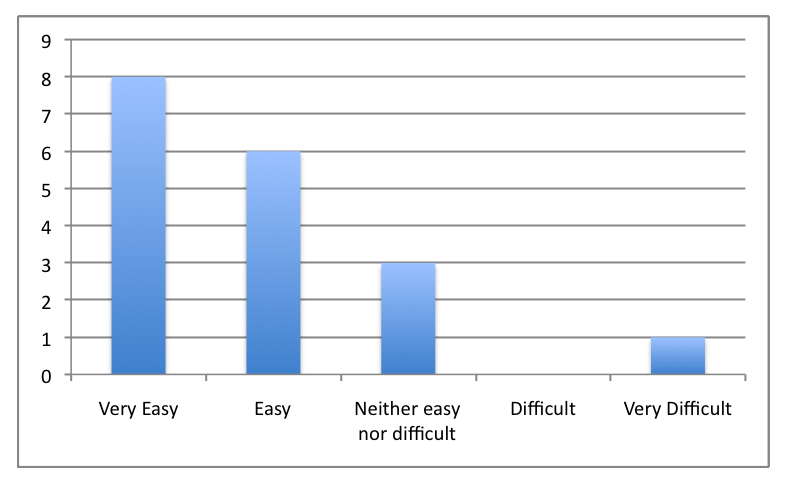
\includegraphics[width=0.6\textwidth]{Q01-InstallEclipseSensor} \\ \hline

2. Installing the Ant sensors (JUnit, SCLC, Emma, etc.) was:
\begin{itemize}
\item Very Easy
\item Easy
\item Neither easy nor difficult
\item Difficult
\item Very Difficult
\end{itemize}
&
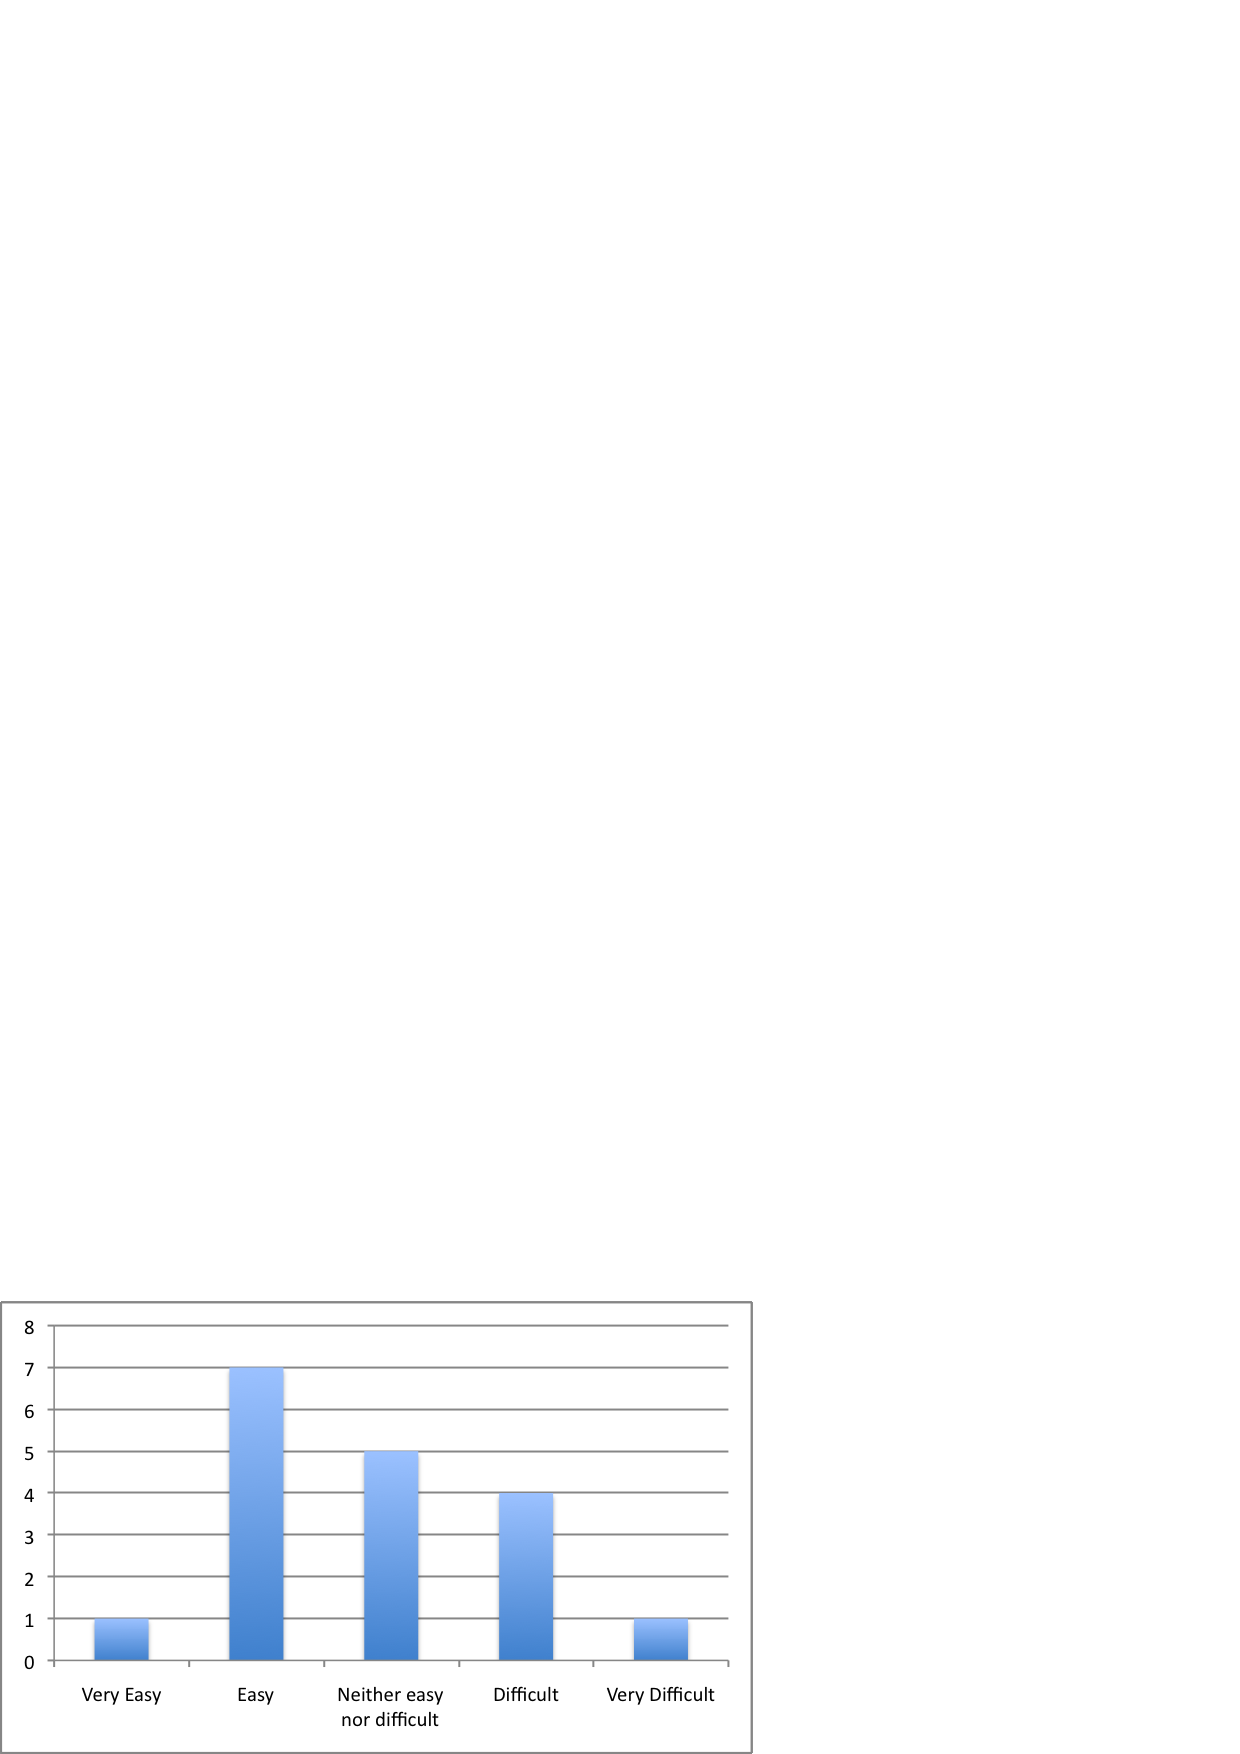
\includegraphics[width=0.6\textwidth]{Q02-InstallAntSensor} \\ \hline

\end{longtable}
\end{center}


3. Please provide any feedback you can on the problems you 
experienced during sensor installation and server configuration, as well as any suggestions you have to make this easier 
in future.
\begin{itemize}
\item I could not figure out what step makes a .hackystat directory. My .hackystat directory automatically generated in my Documents and Settings directory which has a blank space in directory name. I am still not sure how to move this folder to other. The installation of all sensors was pretty well described at the project homepage and there was no problems I have met during the installation. 

\item Both the installation and sending sensor data was easy.  However, tracking down whenever there is a problem with the sensor is not so easy.  A troubleshooting page in the near future?

\item Installing the sensors was pretty straightforward.  I didn't have any problems.

\item Case sensitivity was one problem between user and Hackystat, but it was fixed.  

If it is possible to have a .EXE that will automatically create environment variables and also install files into a local directory will be awesome.

\item I did have one small hang up when installing the Ant sensors: If I remember correctly I was getting a NoClassDefinition error whenever a sensor ran. I was running java 1.5. I fixed it by downloading the jaxb libraries since the errors were referring to that. It could be not related to jaxb at all, but it worked after that. Otherwise, I had no problems whatsoever installing the sensors.

\item Everything went smooth with the instructions given and the verification after each step.

\item Personally I didn't run into any problems but some of the other students did. The sensors aren't difficult to install per se, but there are a lot of steps involved and it's easy to get lost while installing them. Maybe an automated installer can be created that searches for the Ant tools (maybe the user can provide a search directory) and will configure and install the sensors for the user.

\item What made it hard was that all the instructions were not in one page.  I had to go from one page to another and then to another.  There should be instructions from STEP 1 to the end and provide proper links to the step by step process.

\item First of all, the manual is too long. I do like your goal to analyze the software project, but if it wasn't required by this class, maybe I wouldn't think I want to use it, because it looks too complicated. 

Also there are too many things that we need to download and install. If you want to encourage people to use this more, maybe you should provide a package of all the tools somehow. 

For example, before it took a long time to install Apache, MySQL, PHP, and Perl, but now somebody offers a package called XAMPP, which is a combination of all of those, and entire installation finishes in 3 minutes. Something like that should be given. 

\item There is a lot of documentation in a lot of different places.  It was confusing trying to figure out what to read in what order, and whether or not it was relevant to me.

\item Some the installation instructions could benefit from ``write once, use many times'' as they're repetitive, which causes some people to start glossing over the instructions and then there's a couple that are slightly different and people (like me) won't notice the difference.

\item The walkthrough was great, which made the installation easy.

\item The only problem I had was the installation of the Ant sensor. I mean configuring it on Eclipse was easy especially when I try to run Emma, JUnit, FindBugs and all that from Eclipse it is sending stuff to Hackystat but when I checked my software ICU I didn't have any data on Build (all it says was N/A). And little did I know that when you run the ant sensors on Eclipse it only registers all the data to Hackystat JUnit, Emma, Checkstyle and such except BUILD. And I was told  that running the BUILD on the command line works but not on Eclipse. So I tried that and YES that works. So is there a way to make it work on Eclipse when you run all the Ant sensors and it sends all the data to Hackystat including the BUILD data?

\item When we ran the svn sensor, the build would fail if there are any commits from members not identified in our local Usermap.xml.  Instead of looking for all commit records from all users within 24 hours, perhaps it could filter out and only look for records inside our UserMap.xml.

\item The installation documentation must be read carefully.  It may be easier to create a hackystat.build.xml with all the build targets, then import that file into each *.build.xml and call the sensor from the tasks.

\item The most challenging sensor to get up and running was the SVN sensor.  Other than that, the others seemed fairly easy to install.

\end{itemize}

\begin{center}
\footnotesize
\begin{longtable}{|m{0.4\textwidth}|m{0.6\textwidth}|}
\hline 
{\bf Question}&{\bf Response}\endhead \hline
4. The amount of overhead required to collect Hackystat data (after successful installation and configuration of sensors) was: *
\begin{itemize}
\item Very Low
\item Low
\item Neither low nor high
\item High
\item Very High
\end{itemize}
&
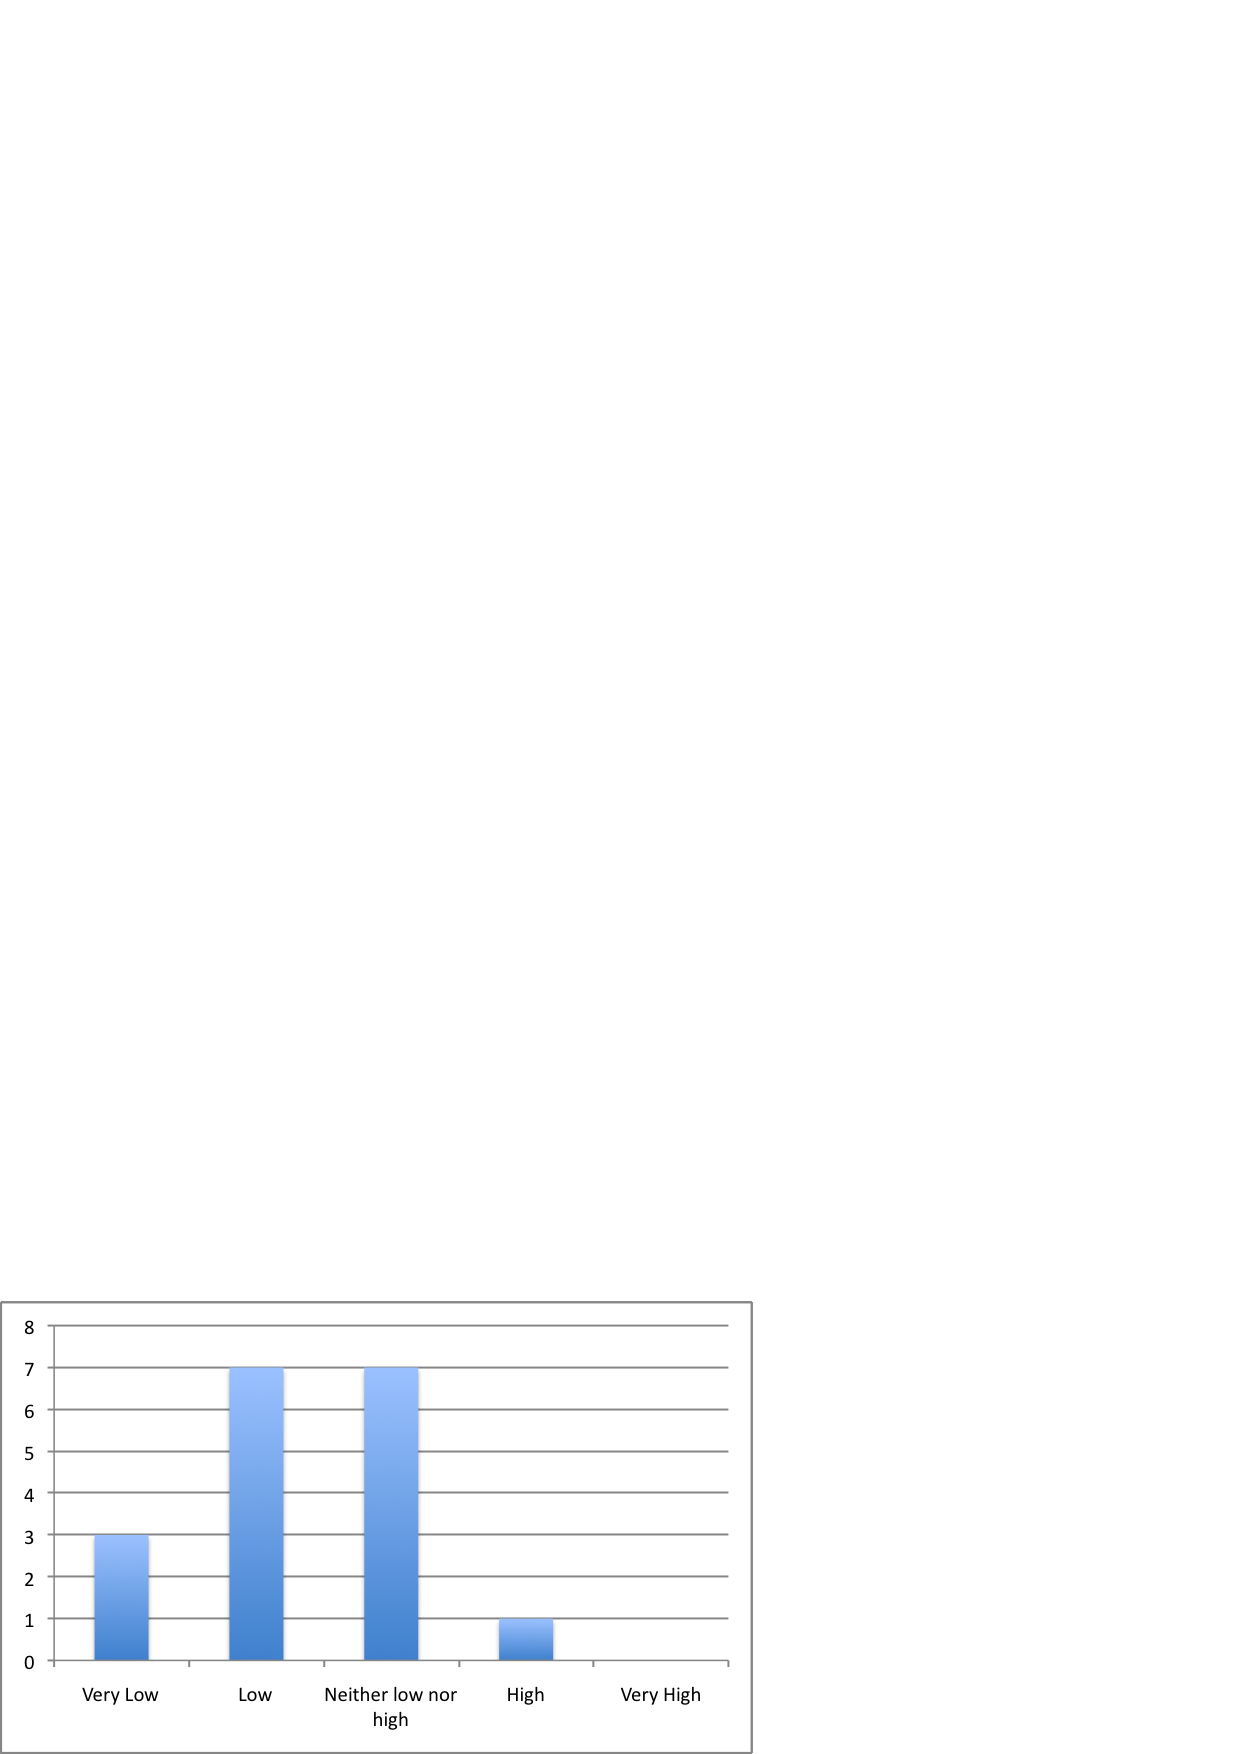
\includegraphics[width=0.6\textwidth]{Q04-DataCollectOverhead} \\ \hline

5. The amount of overhead required to run Hackystat analyses was: *
\begin{itemize}
\item Very Low
\item Low
\item Neither low nor high
\item High
\item Very High
\end{itemize}
&
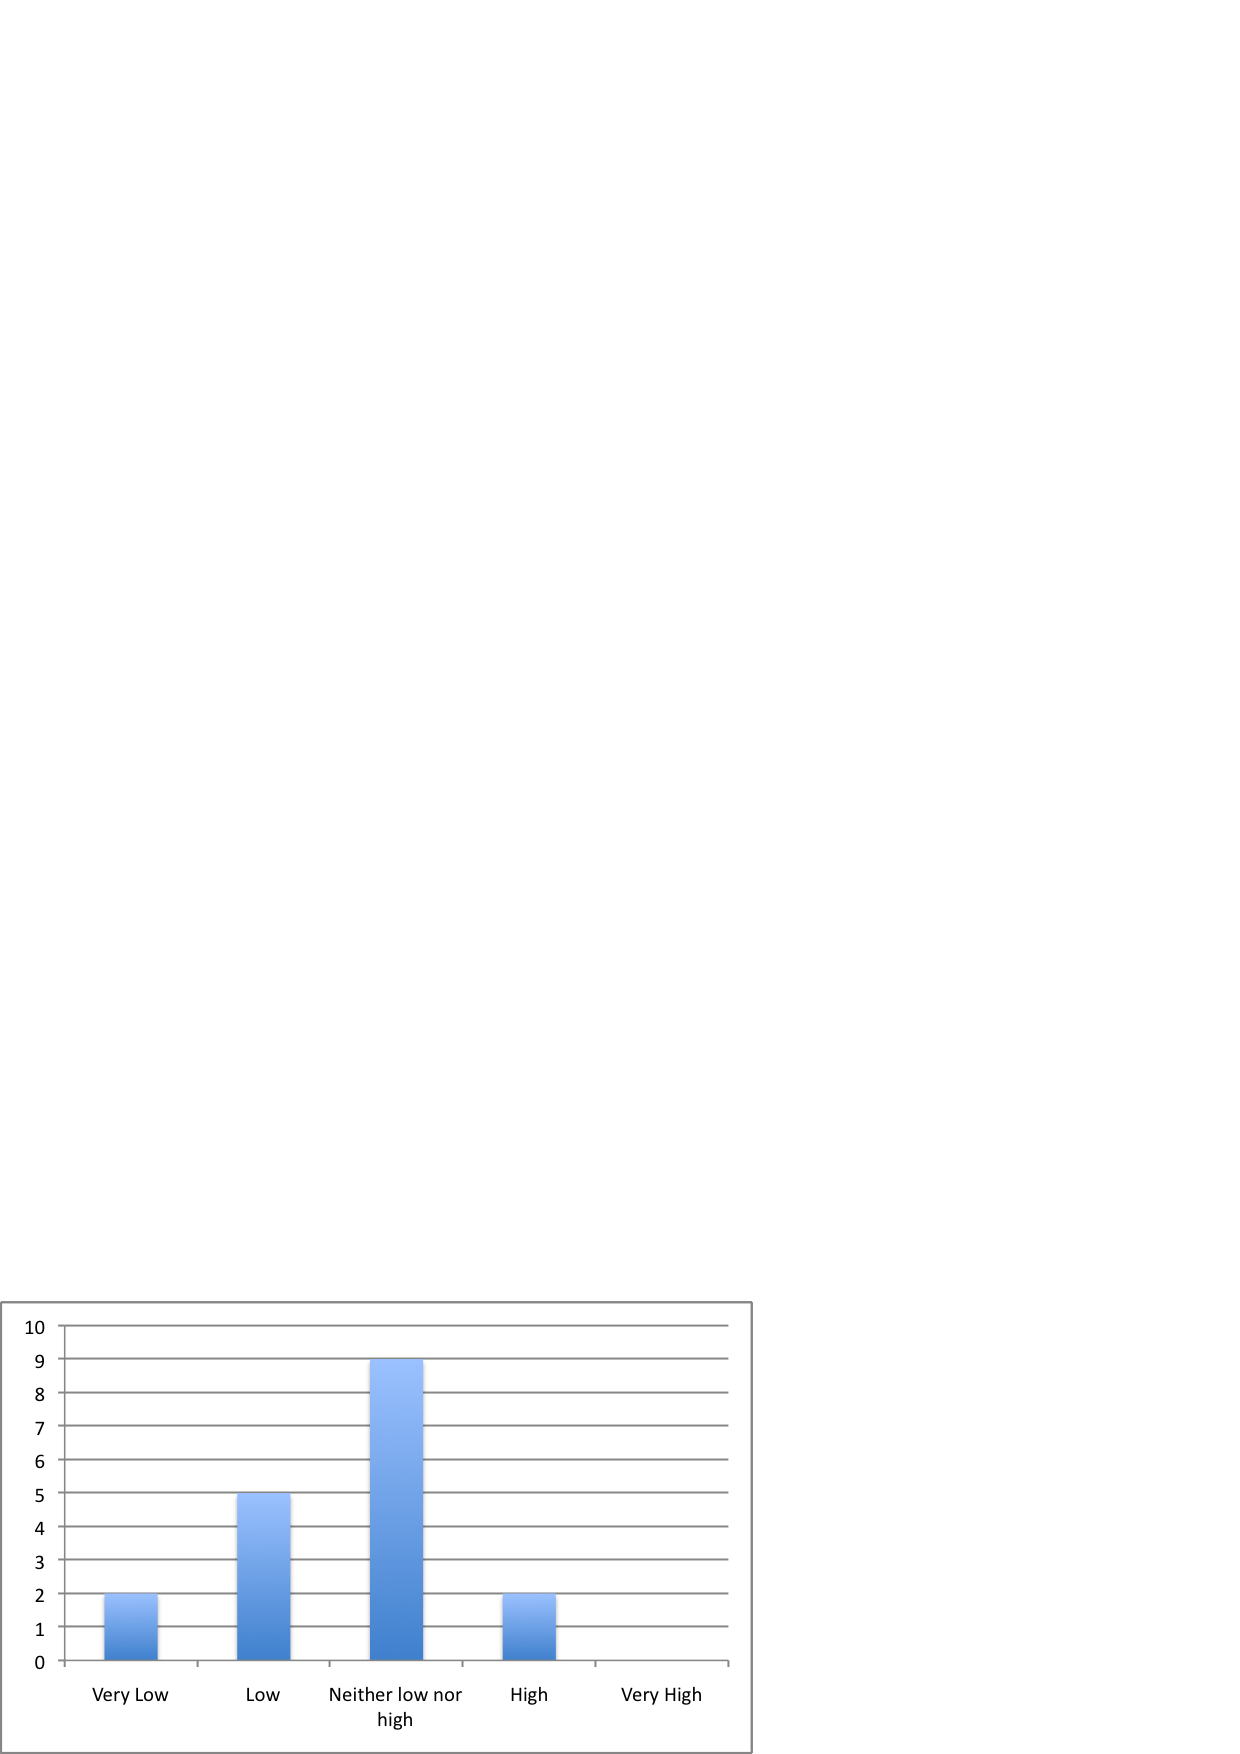
\includegraphics[width=0.6\textwidth]{Q05-AnalysisOverhead} \\ \hline

\end{longtable}
\end{center}


6. Please provide any feedback you can on Hackystat overhead, 
as well as any suggestions you have to reduce the overhead 
in future. 
\begin{itemize}
\item Since the verify command runs all the tests, I'd think that it should send data for all tests run.  Rather, in the portfolio analysis, the Unit Test portion only retrieved data for any JUnit builds that were run.  It doesn't really make sense why we'd have to run it separately when verify does it anyway.
\item If I am correct, overhead - the processing time required by a device prior to the execution of a command.  Then it all depends on what computer the user is using,  I am using a single-core processor laptop it did not take long.
\item Since Dr. Johnson provided us with Ant sensor examples, it was quite easy to set up everything to send data to the sensorbase. I did the hackystat tutorial and everything worked fine. However, I missed the part about creating a usermap.xml file for the svn sensors through Ant. That confused me a bit later on but I figured it out.

What made getting data quite easy as well was having Hudson installed on a dedicated continuous integration server. Daily builds would auto-send data to Hackystat and this made it super easy to get daily info.
\item The sensors ran automatically and it was fast with sending the data.
\item Maybe there can be a link on http://dasha.ics.hawaii.edu to both the Hudson and Hackystat server, that way we don't have to memorize the port numbers. Also, allowing us to create an account and password would go a long way towards usability. I had to put the Hackystat login information in a text file because I can't remember a randomly-generated string for the password.
\item Sending sensor data was often quite slow.  Generating reports in the web application was sometimes also slow -- the page wouldn't load until you refreshed it.
\item The overhead to collect data was generally small, however long enough that would generally run multiple (DOS) terminals so that I could continue working while it was sending data.  Analysis was no overhead since that was just pulling up a browser page.
\item When sending hackystat data, it was fairly quick on my computer, MacBook Pro. Tho, there were some students I saw which had a LONG wait time on the same laptop.
\item I love Hackystat! It is a very great tool especially for a developer like me.
\item Since Ant takes care of running Hackystat sensors, this made it very easy to accomplish. 
\end{itemize}

7. Did you encounter any problems while collecting data? Was 
there any kind of data that you failed to collect? If yes, 
please explain. 
\begin{itemize}
\item I had a problem with sending commit data to hackystat when I worked on a group project. That was because I did not update my sensors to newer version. 
\item At first during the implementation of DueDates 2.0, it was not collecting commit data from my account. It was due to the account on hackystat, it included the @gmail.com part of my gmail account. So it was not matching up with each other, the hackystat account and my gmail account.
\item Running an analyses on my machine was slow, it would take over 3 minutes to run a build.  I am not sure why it took so long to send the build data so I can't make a suggestion.
\item Only JUnit data as mentioned previously.
\item Case sensitivity was an issue at first, but it was corrected so I did not get problems after that.  Hudson did not send to Hackystat number of commits, but that was fixed after a little modification with build.xml file.   
\item I was lucky. I rarely had any problems collecting data during all the time I worked with Hackystat. The one time something got screwed up was with my development time for one day. It said 0 when I checked and I had put in a bunch of time that day so it should have said otherwise. 

I don't remember exactly but, that night I believe had worked in eclipse till after 12 at night, so it went to the next day before I closed the program. That could possibly be a reason for the missing data initially. The next day I just cleared the cache and it was all fine.
\item There was a small issue when I first started collecting data, but it was quickly corrected when checking the xml files.
\item Personally I ran into no problems collecting data.
\item Sometimes it didn't collect build data for some reason.
\item Occasional problems with SVN collection, I think, was a bit hard to tell.
\item Everything was great except collecting data for my BUILD (please refer to above statement for more detailed problem regarding this). Thank you.
\item I did with commit records but it was my fault.  I wish subversion with Google Project Hosting would be more strict.  I was able to check out the project with or without the ``@gmail.com'' suffix (i.e. ``test'' and ``test@gmail.com'').  Thus making me two different authors.
\item Yes, the build data.  I needed to set more environmental variables. 
\item For some unknown reason, my user name picked up the @gmail.com, so both my user name with and without @gmail.com needed to be added to the projects.
\end{itemize}

8. How did you feel about sharing your software development 
data with other members of the class? 
\begin{itemize}
\item We could see how other groups were doing by sharing our software development data with other people. We also could find out what kinds of problems with our project by comparing graphs with other groups and this helped a lot. 
\item I was not offended if it was low, and I was quite intrigued with others data.  
\item I did not have a problem with sharing data with other people in class.  I thought it was needed tool to keep tabs on everyone to assure they're doing their fair share.
\item It felt good if your data was better than others.  And if it wasn't, then you felt bad.
\item Did not really like it because it is showing my programming habits, like starting on a project on the last couple of days.
\item I felt alright about sharing my data with the class. It was interesting for me to see how other people worked on stuff. Some were consistent and others were not. Some people spend a lot of time working on stuff yet do not commit as much as others that work half the time. I think its good to see this data.
\item I am okay with sharing my data.  
\item I didn't think it was a particularly good idea because it then forces group members to become competitive with each other, especially if one person is able to put in more time than all the others. Also, the data doesn't reflect the amount of work put in, maybe someone spent 5 hours doing research and only 1 hour programming, but the sensor data will only show 1 hour of development time and a minor code commit, versus someone who, say, just changes around the package structure for 3 hours and has a huge commit amount.
\item Actually hackystat (or hacky-stalk as what my teammates and I called it) caused a lot of arguments and trash talk.  Some guys were more concerned about collecting stats on hackystat than actually finishing the project.  Some members would start competing on who had more commits or move development time.  The project turned out to be more of a competition of stats, which wasn't healthy for the team at all.
\item It will be obvious that who worked on the project, so it is nice in terms of grading students. At the same time I feel some pressure that I need to work on the development, so if team leader require everybody to work well, this is good.
\item Didn't really care.
\item I had no problem with this, and it encouraged me to be aware of my time management and coding style.
\item It was good in a sense that they can help you with test cases and coverage.
\item It was fun..because you can see how everyone is doing within your group.
\item Before taking this class, I didn't think that there was a way to track software development process. After learning about software continuous integration and working in a larger group project, I have a better insight in sharing the development process. I feel that it is a must in every software development environment, big or small to be able to communicate frequently and effectively. 
\item I was nervous because certain individual of the class seemed able to put in ridiculous long hours.  I was concerned my amount of time (which seemed reasonable) would make me look as though I'm not working as hard. 
\item Good, I can see how I and others rank with each other.
\item I am fine with this.  All group projects in all schools (e.g., Architecture) should be required to use such a system.  This is great for facilitating fair evaluations of students who participate, and those who 'get the grade' by riding on the laurels, blood, sweat, and tears of others.
\end{itemize}

\begin{center}
\footnotesize
\begin{longtable}{|m{0.4\textwidth}|m{0.6\textwidth}|}
\hline 
{\bf Question}&{\bf Response}\endhead \hline
9. How frequently did you use the telemetry page? *
\begin{itemize}
\item Every day or more
\item 2-3 times a week
\item Once a week
\item Less than once a week
\item Never
\end{itemize}
&
\label{Q9}
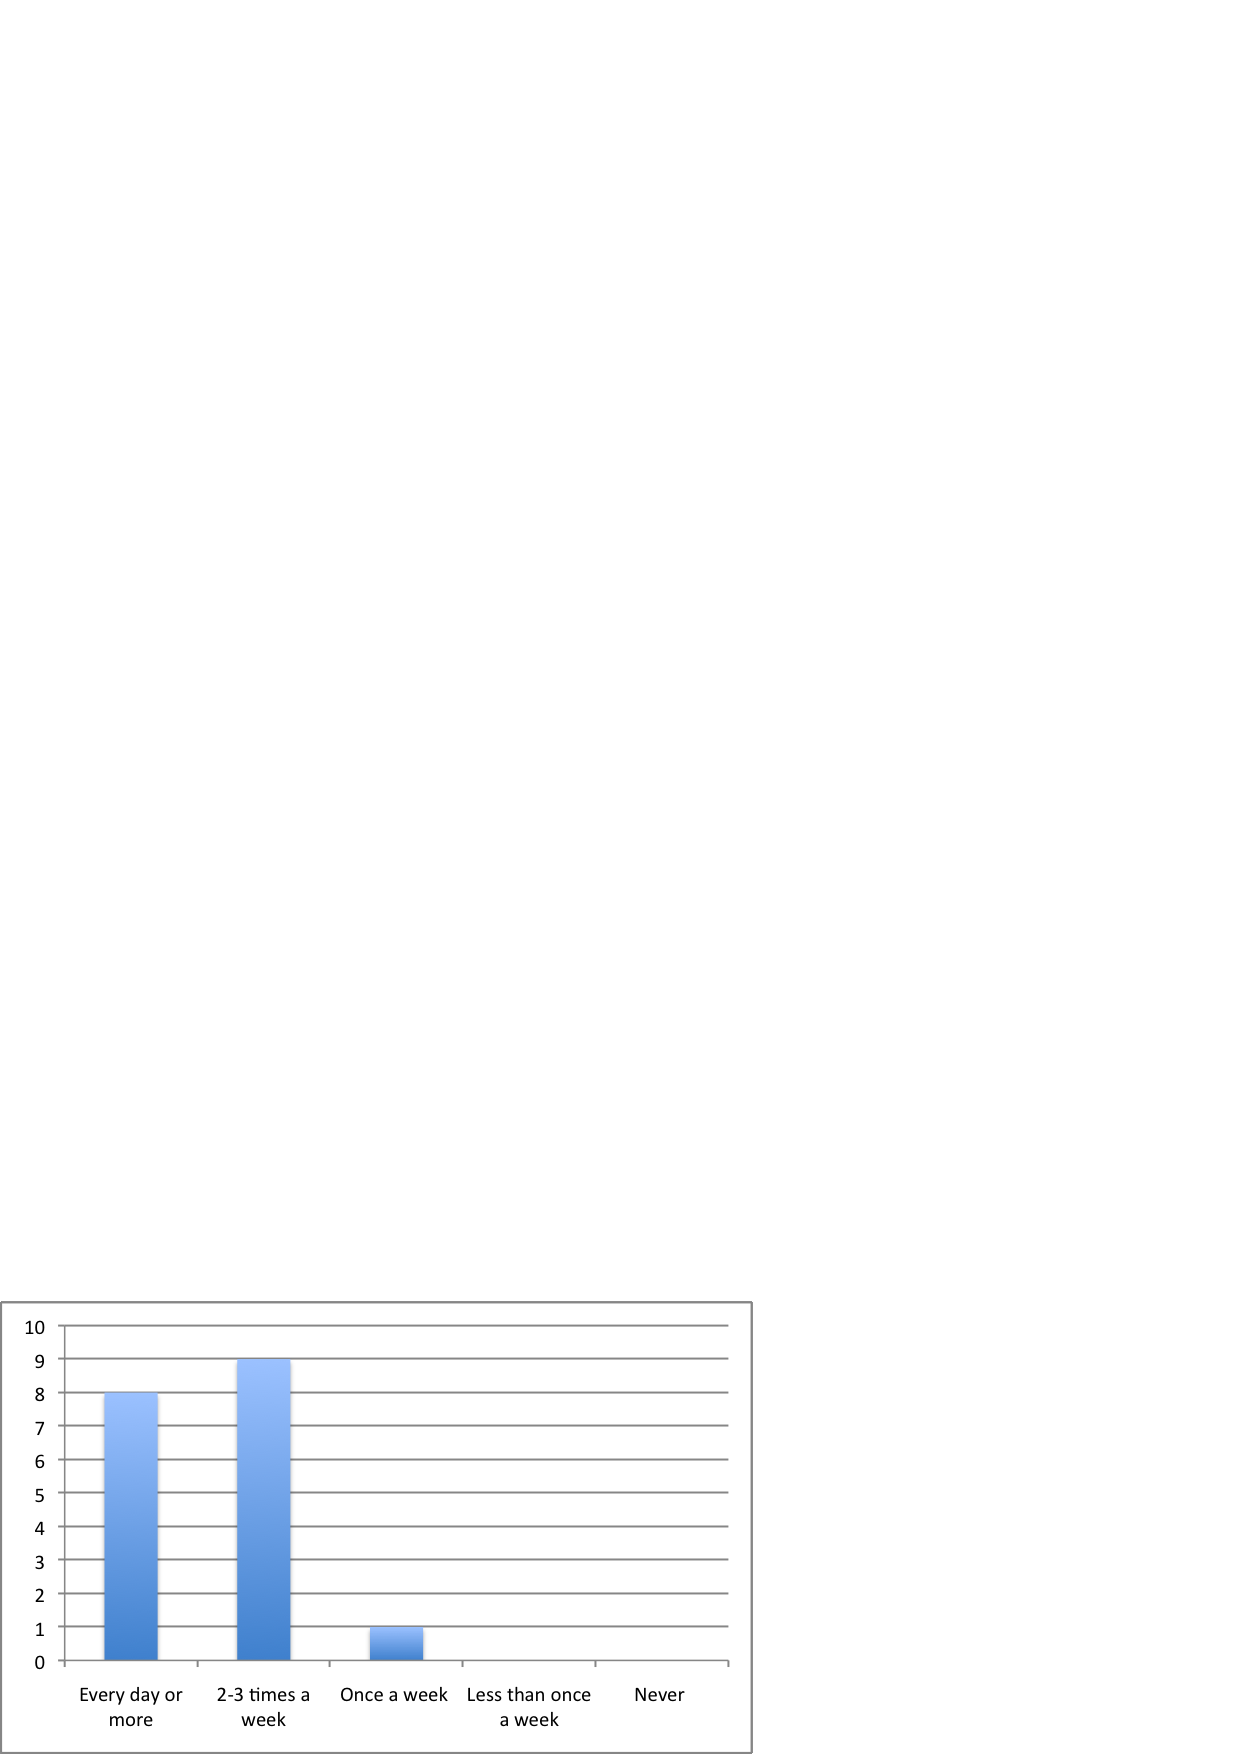
\includegraphics[width=0.6\textwidth]{Q09-telemetryFrequence} \\ \hline

\end{longtable}
\end{center}

10. If you used the Telemetry page, what were you trying to find out? 
\begin{itemize}
\item I tried to find out how was I doing for the project by looking hackystat data. 
\item Seeing how much time i spent on the development of the program, and also others in my group.  
\item When I used the telemetry page I was trying to find out if I was on par with other groups members in terms of development, build, and commit numbers.
\item Whether or not, my sensors were reading, and the work output of my group members (especially on days we didn't meet together).
\item If my development time was up to par with my team members.
\item I usually used the telemetry page to evaluate how my team was working overall, and what my part was in that data. I also checked it to make sure everyones data was being sent.
\item It helps me see how I measure up with my partners.
\item Member dev time mostly, to compare the amount of development time I put in vs. my group members.
\item It supposed to show us how healthy individuals are in the group. So if one person is slacking, the members need to tell him to step it up.  It wasn't used that way in our group.  One person really wanted a good grade for the class so he just used the telemetry to watch himself; making sure no one gets more builds/devTime/commits than him (yes he said ``i need more dev time because i need an A'').  I remember we had dinner as a group and one of our group members didn't go to dinner.  another group members then said ``oh if he ups his stats more than mine, tomorrow I'm gonna hack all day.''

Sad, but true.
\item member commit, member dev time
\item Curious about trends in dev time, commits.
\item Usually MemberDevTime, MemberBuilds, and MemberCommits.  Basically just seeing how everyone was progressing.
\item graphs, line trends of other group members
\item My status and the status of our group and make sure everyone is doing their part.
\item Mostly trends in individual performance, as well as overall project outlook.
\item Basically if everyone was putting in the same amount of effort.  Also it helped indicate if everyone is on track.  If they have regular activity, then the chances of them on track is higher.  
\item Was the coverage, complexity and coupling getting bad?
\item I tried to review each telemetry page daily to understand what I could do to improve the project health and focus efforts.
\end{itemize}

\begin{center}
\footnotesize
\begin{longtable}{|m{0.4\textwidth}|m{0.6\textwidth}|}
\hline 
{\bf Question}&{\bf Response}\endhead \hline
11. How frequently did you use the Software ICU? *
\begin{itemize}
\item Every day or more
\item 2-3 times a week
\item Once a week
\item Less than once a week
\item Never
\end{itemize}
&
\label{Q11}
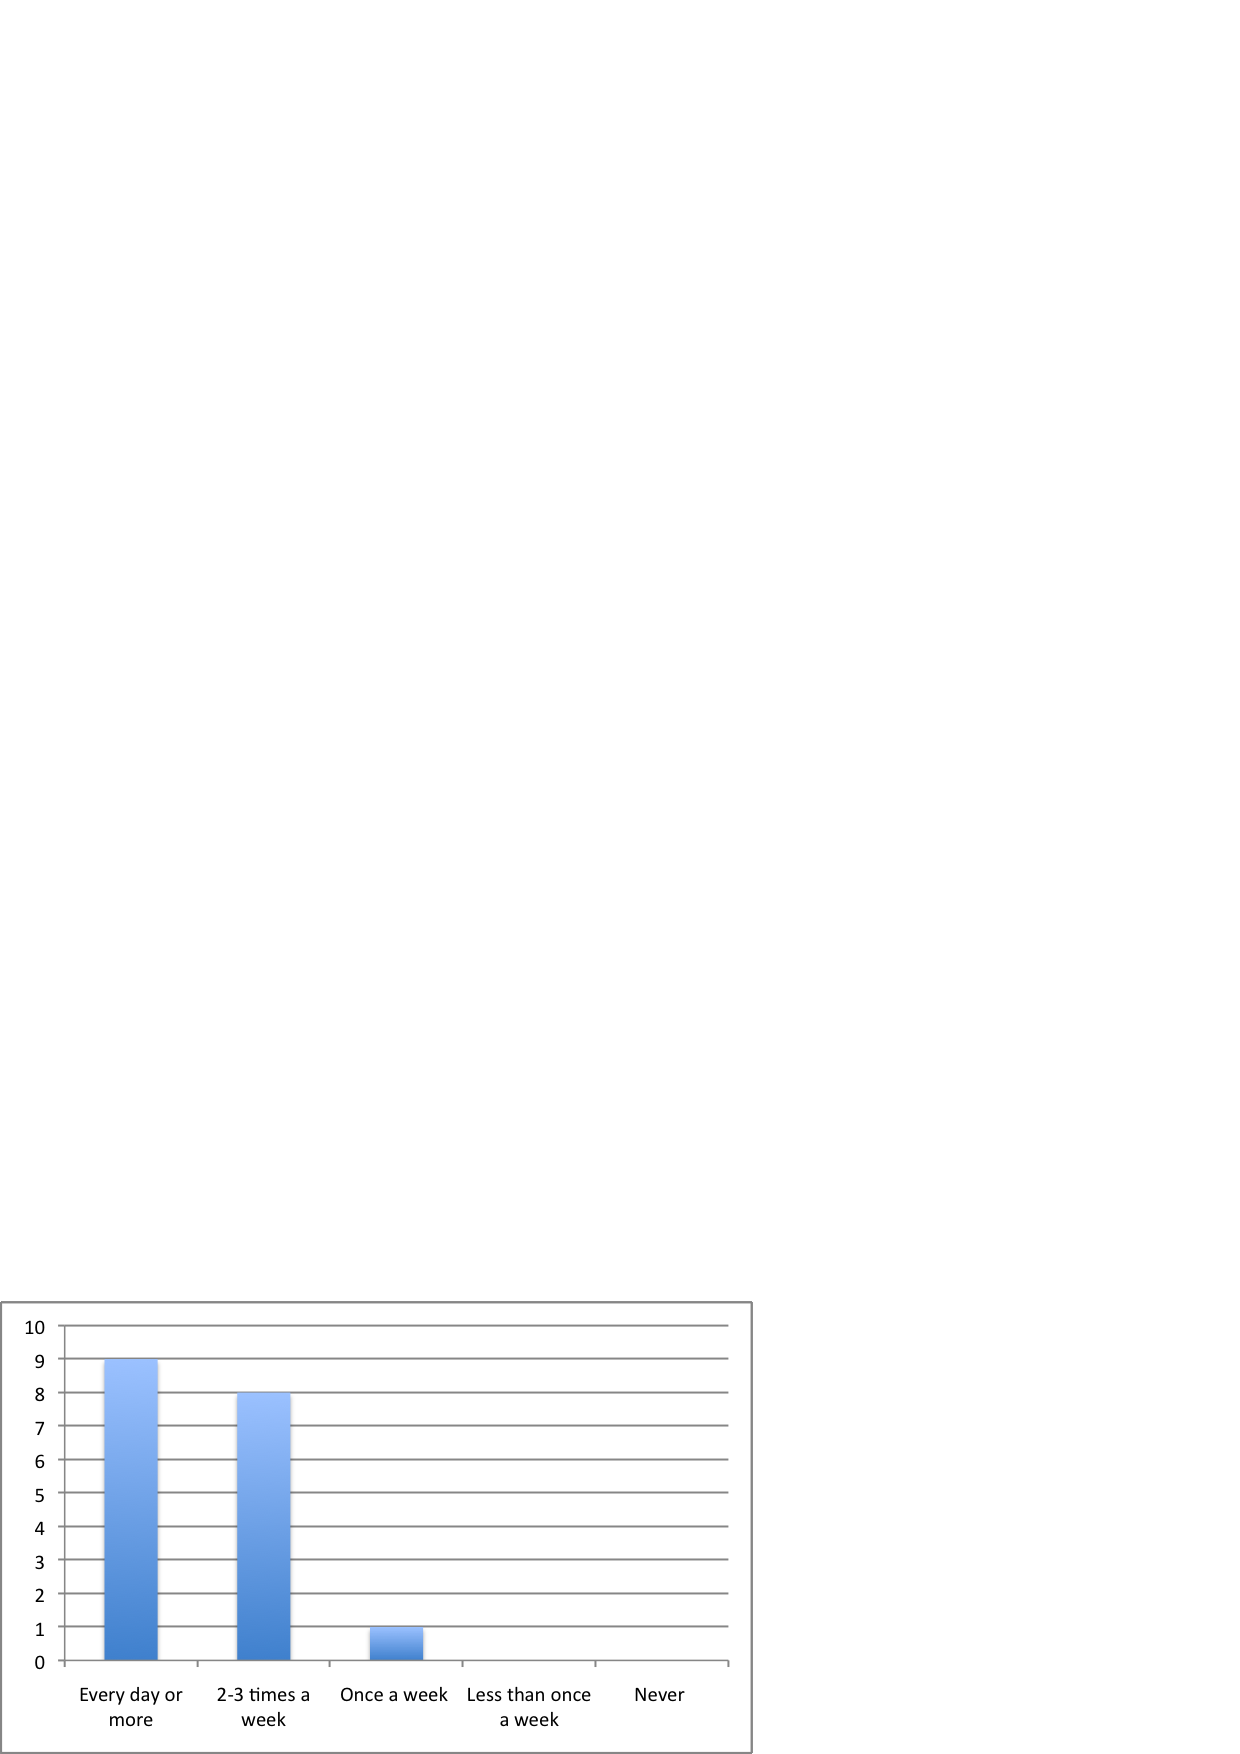
\includegraphics[width=0.6\textwidth]{Q11-ICUFrequence} \\ \hline

12. If you used the Software ICU, please check the vital signs that were useful to you. *
\begin{itemize}
\item Coverage
\item Complexity
\item Coupling
\item Churn
\item Size
\item DevTime
\item Commit
\item Build
\item Test
\item None of the above
\end{itemize}
&
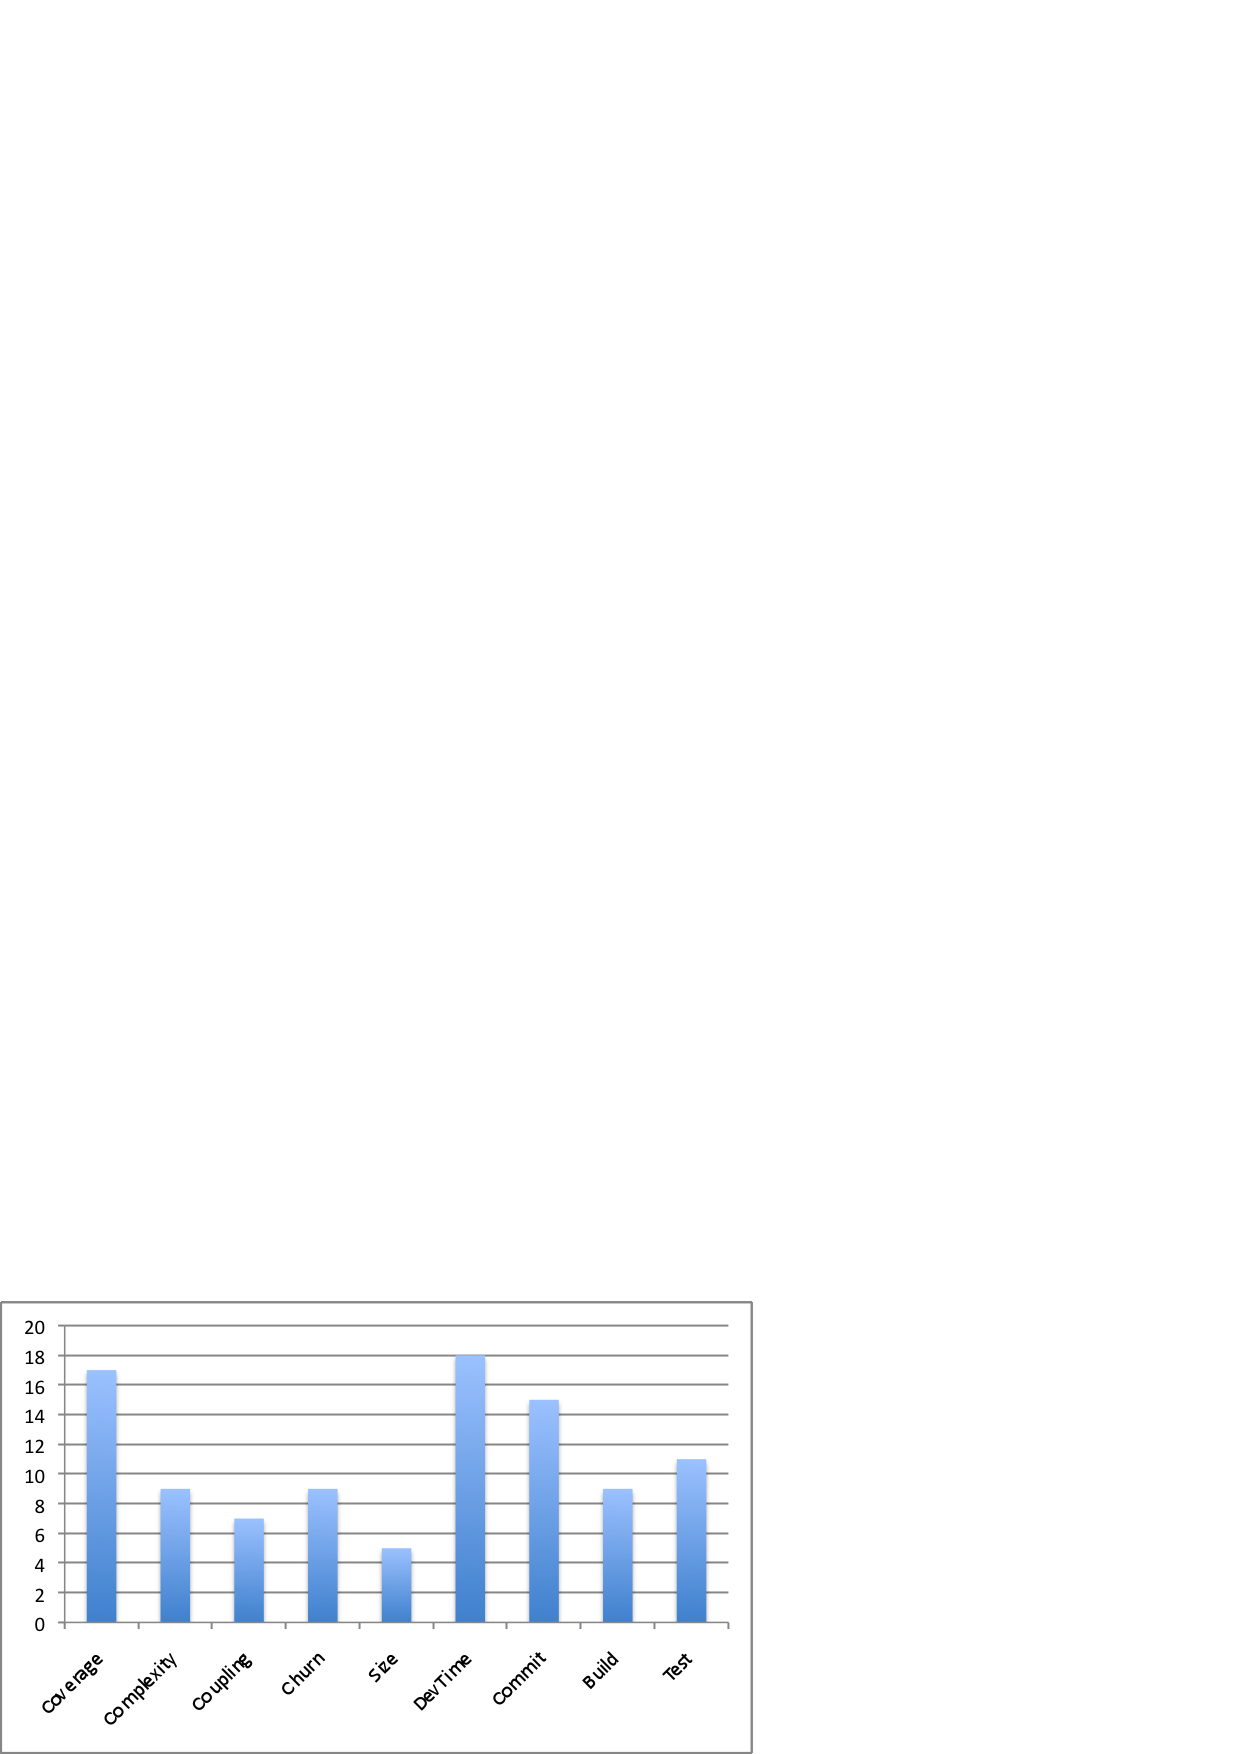
\includegraphics[width=0.6\textwidth]{Q12-UsefulVitalSigns} \\ \hline

\end{longtable}
\end{center}

13. Did you feel the Software ICU colors accurately reflected the health of your project? If not, why not? 
\begin{itemize}
\item I felt most of colors accurately reflected the health of the project. For the Coverage data, since we can write test cases just for increasing of the rates, we cannot assume that the project is in healthy condition even if the coverage data displayed in green color. However, I think this is not a problem of hackystat. 
\item Yes
\item The only issue I had with the ICU colors was with the coupling.  In both versions of DueDates we had to add extra classes at the last minute which would cause the coupling ICU to turn red.  I am not sure how to address that because the coupling does need tracking.
\item Not really, I don't think having a high churn amount is necessarily bad.  Of course, it's a case-by-case thing.  For my group, it wasn't about not committing frequently; we were just rehashing code because something just didn't work.
\item Yes, reflected accurately on the health of the project.  Showed how much coverage we had.
\item I feel that the Software ICU did accurately reflect the health of my projects. For Due Dates 2.0, which was a longer project, the data was getting increasingly more meaningful as the trends were over a larger period of time. It is good to look at things like devtime, commits, coupling, and coverage to see the color and the past trend because i think they really say something about the current state of the project.

To make it simpler, whenever I knew our project wasn't doing good and people weren't working regularly, the software ICU would have lots of reds and yellows. When I knew the project was doing better and people were working regularly, there were greens. It makes sense.
\item The ICU was accurate with our project because it showed drastic spikes in all signs.  This reflects our project in poor health.
\item Not particularly because a project's health cannot easily be determined by just measuring numbers alone. For example, it's easy to increase coverage, but if a class has nothing but getters and setters and a toString method, does it really need to be tested? Of course not, but someone might feel compelled to do it in order to increase coverage and get a better health, but it's just a waste of time in my opinion. Also, DevTime is only measured from Eclipse but that doesn't measure things such as someone reading a book or looking up websites for information. It only measures active development in one program, forcing people to only use whatever IDE's Hackystat supports. The figures for complexity and coupling are hard to evaluate too. We want complexity to be low but sometimes it's unavoidable for it to be high, and should Hackystat show an absolute cut-off point where the complexity must be below a certain point for the project to be considered acceptable? Coupling is another one that falls under this category, if your program relies on a lot of outside libraries, can someone really determine an absolute value that the project's coupling must be under?
\item Yes.
\item maybe
\item Coverage: perhaps too sensitive to drops/bounces in coverage.
Churn: while you're working on a project, churn is going to vary, sometimes a lot.  The trend colors were not helpful.
\item Yes, I felt it was a relatively healthy project, and this generally showed, in the end.  In the first half the colors reflected not as health of a project, which I'd agree as well.  I'm not sure rising coupling was entirely a bad sign as things went along and functionality was added, as it was a slow steady rise.
\item Sometimes.  Hard to determine what will fall into green, red, or yellow.
\item Yes definitely.
\item It somewhat reflected the quality of our project. Maybe in some dark corner something is not thoroughly being depicted through the colors. Perhaps a suggestion is to use different color hues.
\item Yes it was pretty accurately reflected.
\item No, since I did not correctly configure the sensors.
\item This is subjective...  Usually the colors were spot on, however, they are quick to turn one way or the other depending on events that are being managed by the team (e.g., large code churns due to removal of unused code/imported code, etc.).
\end{itemize}

14. Were you able to use the Software ICU to improve your software's quality and/or your team's process? If so, in what ways? If not, why not? 
\begin{itemize}
\item We can check how other members are doing for the project through the Software ICU and this helps a lot especially when we are working on the team project. 
\item Yes, for tracking if members were working on their tasks. Also how complex the program is increasing or decreasing. 
\item In my opinion, it is not clear if the ICU improved our system.  Because other tools such as junit, findbugs, and pmd was easier to use to improve the application.
\item If anything, keeping an eye on coverage helped us look out for what was being tested and what wasn't.
Yes, showed how much coverage we had, and improve on that.
\item I think for sure the Software ICU improves team process. More than just keeping people ``in check'' when grades are at stake, it provides an accurate way to assess what's being done and by whom. Our team got a lot out of checking up on the software ICU and assessing our team process. It seemed to get better over time.

As far as the software's quality, I think the Software ICU could be very useful in improving this. If my project for instance was in the red for complexity and coupling, and there were some code issues, I could see all this automatically through hackystat. Besides coverage stats though, my team did not really use the ICU to improve the software's quality.
\item ICU was able to help us because it told us what needs to be focused or corrected.
\item Personally, I only found Hudson useful because it's like running your code on someone else's computer to see if your environment is set up differently from a generic machine. I feel that the data for Hackystat is more something to look at out of curiosity rather than something to determine how well a project's status is because it's hard to base a project's health based on numbers alone and it might put unrealistic pressures on the team to make the project healthy for Hackystat when they can better spend their time developing instead.
\item Yes.
\item Yes, coverage tells me if we didn't write enough test cases.
\item No.  
Coverage: already aware from Emma.  
DevTime, Commit, Build, Test: either team members did not look at the statistics, or they didn't care, because their habits did not change much.
Others: not much we could do about the other statistics.
\item Yes because able to manage our time and development fairly equally, and also notice spikes indicating bigger changes or problems.
\item Yes, shows were we could improve as a group and improve as a programmer.
\item Like in my case last time, I saw on Software ICU that I don't have a data on my BUILD. So because of that information I know what the problem is and it helped me to find a solution and figure everything out before it is too late.
\item Our project ICU definitely described our lacking and late attempt to improve coverage. Due to the ICU, we were able to distinguish this fact quick and easy. 
\item The amount of activity helped us identify who was falling behind.  Without offending our members by outrageously claiming their not working, we could tell by the sensors.  Members can be more self-critical by looking at their individual data compared to the groups.
\item Yes, by checking the coverage, complexity and coupling.
\item Yes.  By targeting coverage, dev time, coupling, and complexity, my team was able to improve all these into areas that were acceptable to us.
\end{itemize}

15. Please provide any other feedback you would like regarding 
Telemetry and the Software ICU, as well as any suggestions 
you have on how we can improve the system. 
\begin{itemize}
\item I do not think the commits, builds, tests should be colored in because it all depends on how much the user does on the project.  Is it possible to show line coverage instead of method coverage? The software ICU and telemetry was awesome tools in helping out with the project.  It gave me visual stats on the project.
\item What I think would be cool is to implement something to view the trend for each category in larger format but in the same style as the software ICU. I know this is shown on the telemetry page when you select it to show. However, I would be nice if there was some sort of rollover function that brought up a slightly larger window with a blown up overall trend. I can see how this isn't really needed but I would mostly likely check it a lot if it was there. 

A minor thing that I noticed when using the Telemetry page was that when I selected a new statistic to view, the page would always jump back to the top and I'd have to scroll down each time. Its not really a biggie, but it makes navigating a bit slower when your going through all the project statistics.
\item Consistent colors for each members can help.
\item In addition to everything I mentioned above, it might help to somehow make the sensors configurable in some way, for example if two people are doing pair programming, there should be an option to set the sensors to send data for both people. Perhaps complexity can be measured somehow to only include methods that, say, start with get or set and toString. This way people aren't forced to write pointless test cases in order to increase coverage. 
\item Help page should be provided inside project browser. It should describe how to use it, what telemetry, what churn is, something like that. 

Also your explanation should be simple so that people want to read it. If it is complicated and long explanation, nobody will read it. 
\item The different color bars and randomness might be fun and interesting, but I think having a bit more consistent scheme might be better.  I would suggest if possible giving each developer a specific color that they always have during the project, either random, or chosen at the beginning.
\item Does not capture development outside of Eclipse.  For example, IMHO, MS Visual Studio is much better in the capacity as a web development IDE, which the dev time here was not recorded.
\end{itemize}


\begin{center}
\footnotesize
\begin{longtable}{|m{0.4\textwidth}|m{0.6\textwidth}|}
\hline 
{\bf Question}&{\bf Response}\endhead \hline
16. If I was a professional software developer, using Hackystat at my job would be: *
\begin{itemize}
\item Very feasible
\item Somewhat feasible
\item Neither feasible nor infeasible
\item Somewhat infeasible
\item Very infeasible
\end{itemize}
&
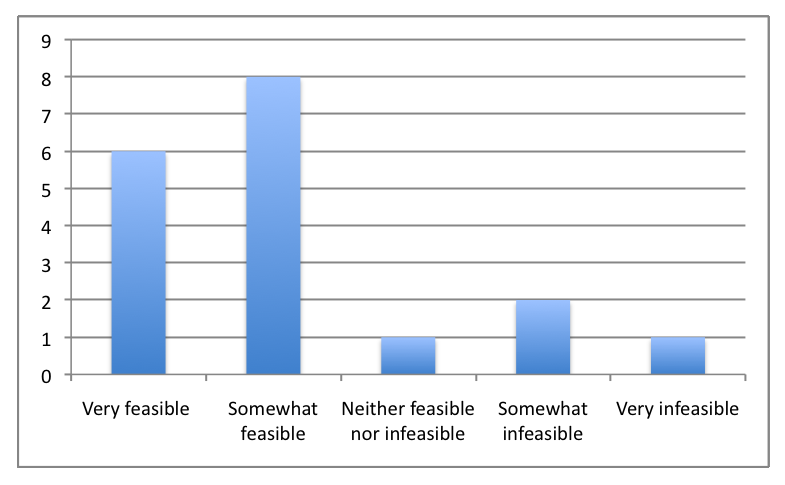
\includegraphics[width=0.6\textwidth]{Q16-FuturePredict} \\ \hline

\end{longtable}
\end{center}

17. Please provide any other feedback you can on the feasibility of Hackystat in a professional setting, as well as any suggestions you have on how its feasibility could be improved.
\begin{itemize}
\item I think it's good to have this in a professional environment, cause the employer or client  can check on how the progress of the program is going. With out having to make so much visits or hovering over workers.
\item Cannot think of any off the top of my head.  The Software ICU is already great for us programming students.  
\item I think Hackystat is definitely feasible in a professional setting, as long as it is supported in some way. For instance, if a team of developers is working on a project and they are all for having Hackystat manage project stats, that would be great. If, however, your the only person on your team that wants to use it, then it would be hard to send data that would assess team process.

I could see project managers wanting to have Hackystat data to evaluate everyone's input into the project, as well as the health of the project. Hackystat, I think, is perfect for new open source projects if releases are made early and often. It could be essential to seeing the overall health of the project.
\item Overall, I feel like Hackystat would be an interesting tool to gather data to look at for curiosity's sake from time to time, but it should not be used as a basis for determining a project's health or to determine something such as member contribution. The sensors can only gather information from a few sources and these readings cannot account for a person's full contributions to a project. As for determining a project's health, I do not believe the sensor readings can provide an accurate measurement because the sensors can only measure numbers based on algorithms, but it takes a person to really determine how good the code is.
\item When I start to use hackystat, I need to get password from you and then eclipse send my data to your server. Some developers might have concern that hackystat steal source code.
\item I think it depends a lot on the culture of job setting.  I'm not too sure, but I think I may try setting it up on my own job site, even if just for myself to see my own trends.
\item It is a very useful tool to keep track the health of a project so I would say it is feasible to have it in a job.
\item My only wish is that ICU's should have a feature to support pair programming. Possibly a feature to indicate to the system that two people may be working on the same problem on the same system, rather than two individual machines. You might want to call this ``collaborative mode'', or something along the lines of that. These settings of course should be turned on or off easily from the developer's IDE (Eclipse).  
\item I work in a one person shop, so it would be difficult to say how useful this would be.  As a lone developer, many metrics I am very cognizant of, however, having such a system would allow me to view those statistics that I do not have a ``gut'' feeling for.  It would be great for my boss to measure the amount of time I spend on a project however.
\end{itemize}

%%% Input file for bibliography
\bibliography{csdl-trs,hackystat,psp,sz-ms-thesis}
%% Use this for an alphabetically organized bibliography
%\bibliographystyle{plain}
%% Use this for a reference order organized bibliography
\bibliographystyle{unsrt}

\end{document}
